\section{Results and Discussion}

\subsection{General Findings}

\begin{itemize}
	\item Noise, which interprets cooperation as defection decreases cooperation drastically.
	\item Noise, which interprets defections as cooperations increases cooperation, but the effect is weaker.
	\item Perfect information is not what’s best for the system. If decisions are transmitted better than they are, the whole system gets more efficient.
	\item Friendly, which means cooperative, players performance drastically decreases if the chance that cooperation is transmitted correct is less than $100\%$.
	\item Players that do not react immediately to defections look non-responsive.
\end{itemize}

\subsection{Problem caused by unreliably transmitted Cooperation}
Many of the friendly players perform well without noise, because they have an infinitely long sequence of mutual cooperations with other friendly players. Noise will trigger defections. This state requires then a way to come back into cooperation. Most cooperative players do not have a mechanism to reestablish cooperation if it has been destroyed once, because they rely on a cooperation caused by the first turn decision being cooperative. 

\subsection{Benefit caused by unreliably transmitted Defection}
Some players try out defective moves. For \verb0TFT0 mutants this can likely result in mutual defections. A noise that inserts cooperative moves results in the \verb0TFT0 player reacting cooperative again, driving the game in mutual cooperation again. Another thing is that hiding defections allows aggressive players to exploit players that would retaliate otherwise, and an aggressive player exploiting a weak one is better than if both players are defecting each other.

\subsection{Axelrods Recommendations}
Axelrod proposed a certain behavior to be successful \cite{axelrod}. This behavior is known as:
\begin{itemize}
 \item     Be nice: cooperate, never be the first to defect.\\[-6mm]
 \item Be provocable: return defection for defection, cooperation for cooperation.\\[-6mm]
\item Don't be envious:: be fair with your partner.\\[-6mm]
\item  Don't be too clever: or, don't try to be tricky.\cite{recon}
\end{itemize}

Under noise$1$ the opponent will see defections from a player, even if he never defected. This diminishes the use of being nice. It is more successful to find out if he responds to defections and exploit the opponent if he is exploitable. In Axelrod's Tournament this was not the case, because this attempt might have long lasting effects. However noise somewhat covers up the past. The other recommendations still hold.

\subsection{The Performance of each Player}

The performance plots shows the average reward of a certain player, depending on the two noise levels. The simulation was run twice, to check for the stability of the results. Therefor, each player has $2$ performance graphs.\\

For some of the players there are tables, which show how many of their moves are cooperative, dependent of the noise levels under which the simulation was run. 

\subsubsection{Cooperative Player}

The player's performance is shown in figure~\ref{Pic Cooperative Player}.\\

\begin{figure}[h]
	\caption{Reward plot of COOP}
	\label{Pic Cooperative Player}
\begin{minipage}[hbt]{0.65\textwidth}
	\centering
	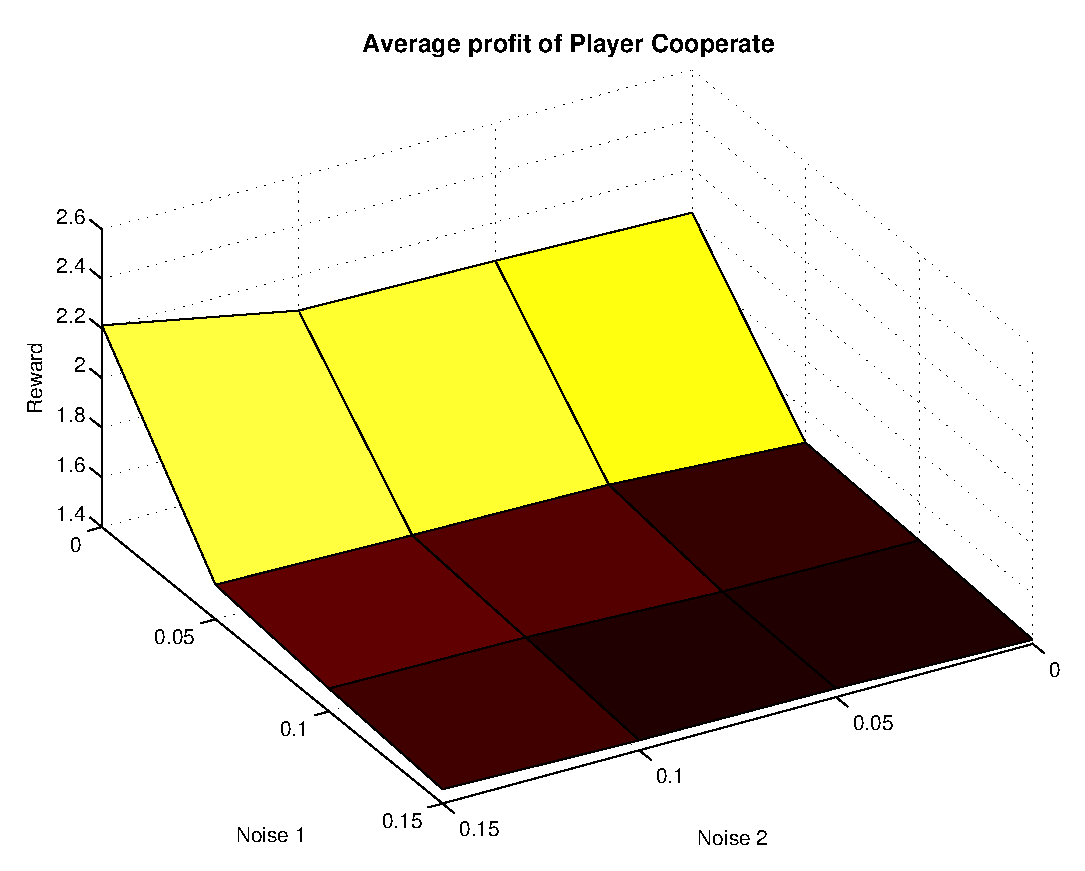
\includegraphics[width=\textwidth]{pics/simulation1/Reward_vs_Noise_of_Player_Cooperate}
\end{minipage}
\hfill
\begin{minipage}[hbt]{0.3\textwidth}
	\centering
	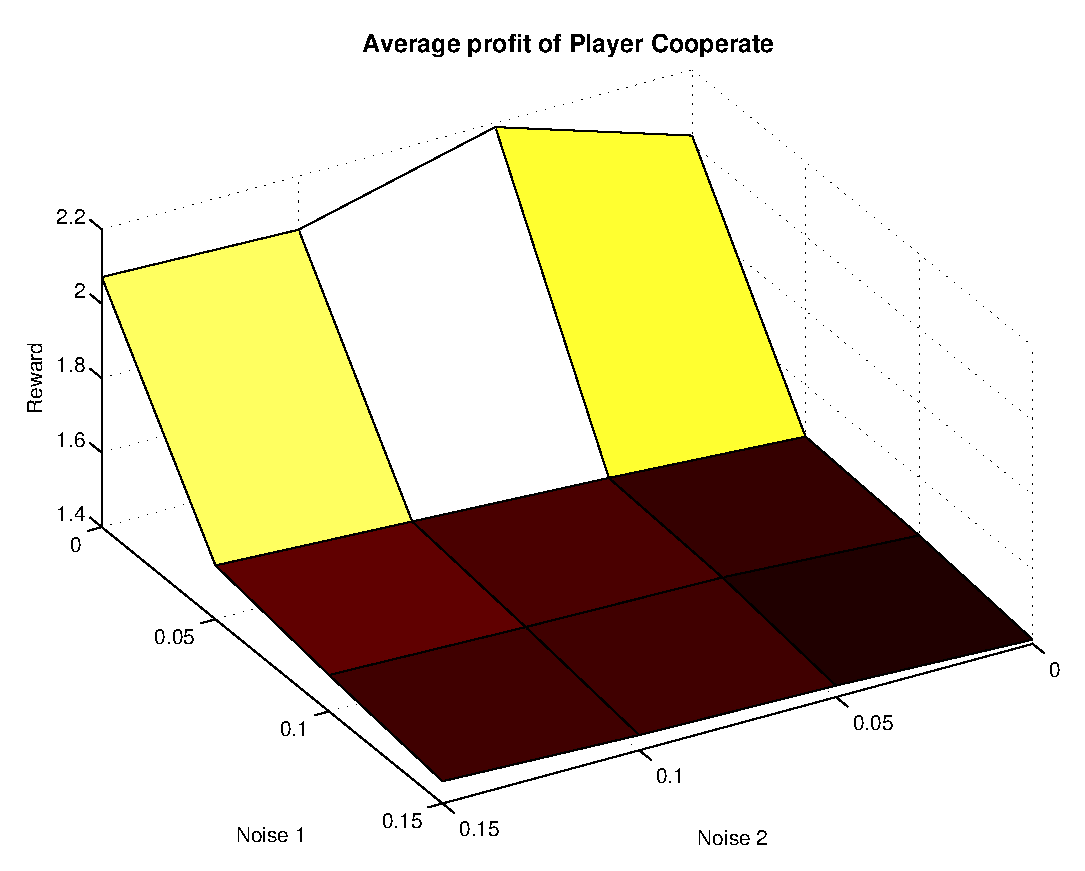
\includegraphics[width=\textwidth]{pics/simulation2/Reward_vs_Noise_of_Player_Cooperate}
\end{minipage}

\end{figure}

In a situation of no noise, this player performs strong against mostly friendly players, but gets exploited by aggressive players. In this situation it performs better than always defect, but similar to random.\\

Because this player is cooperative and not reactive noise$2$ doesn't matter. On the other hand performance drastically decreases with noise$1$. The seemingly inserted rejections make other players explore defective moves. Because the defective moves are not retaliated the other players might then stick with these defective moves. Players that start exploiting this player are \verb0FRI0, \verb0PAV0, \verb0CDO0 and \verb0LCDO0.\\

In a situation with noise this strategy is still strong with \verb0TFT0 mutants, because a cooperative interaction gets restored in the fastest possible way.\\

Still with a drop of $0.7$ to $0.8$ in performance this player is one of the players that is the most susceptible to noise overall.\\

Traits of the player:

\renewcommand{\labelitemi}{}

\begin{itemize}
	\item + Can sustain cooperation with friendly players even in noise
	\item - Exploitable
	\item - Does not respond to the opponents move
\end{itemize}
\renewcommand{\labelitemi}{$\bullet$}

\subsubsection{Defective Player}

The player's performance is shown in figure~\ref{pic player defect}.\\

\begin{figure}[h]
	\caption{Reward plot of DEF}
	\label{pic player defect}
\begin{minipage}[hbt]{0.65\textwidth}
	\centering
	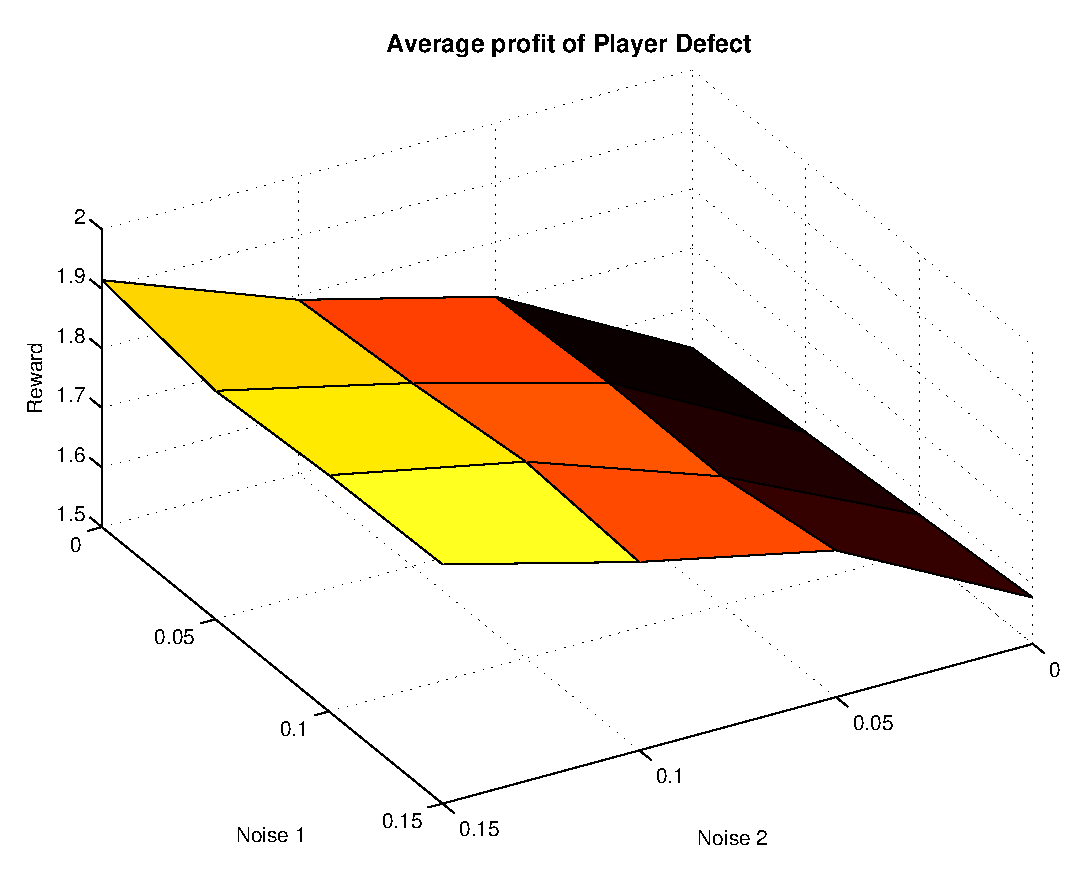
\includegraphics[width=\textwidth]{pics/simulation1/Reward_vs_Noise_of_Player_Defect}
\end{minipage}
\hfill
\begin{minipage}[hbt]{0.3\textwidth}
	\centering
	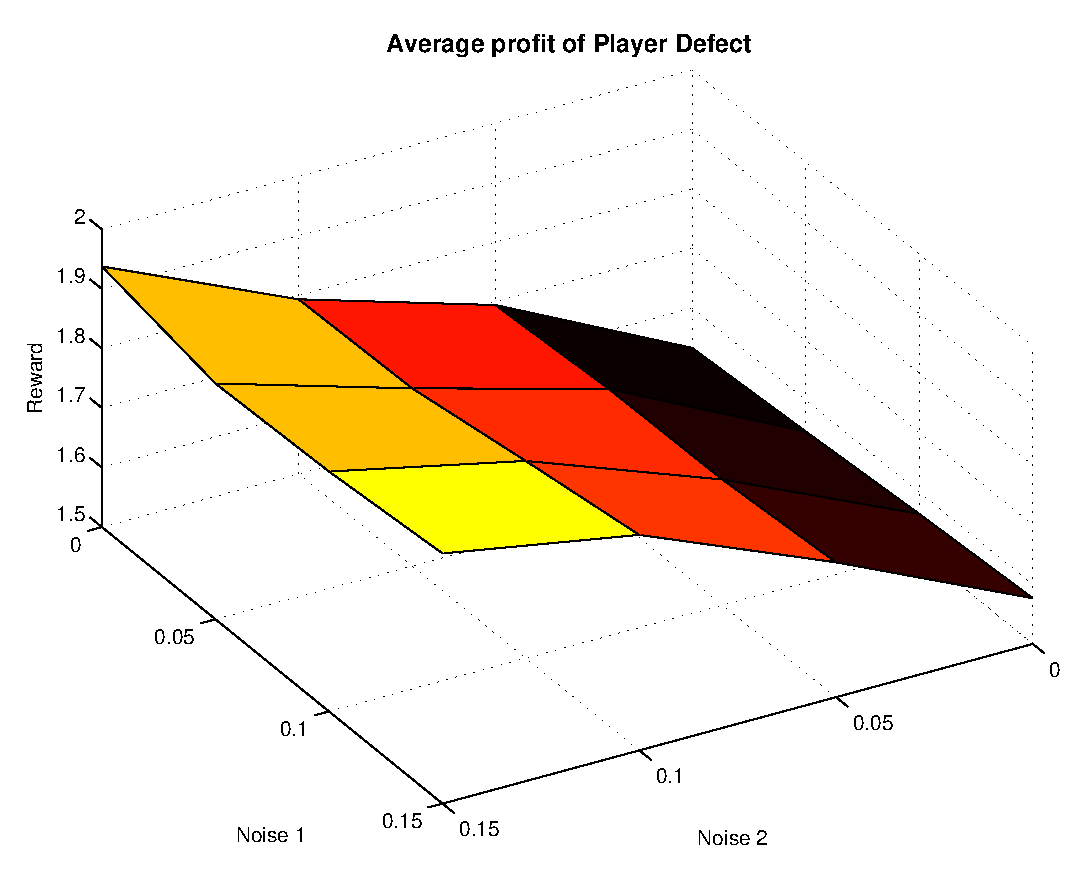
\includegraphics[width=\textwidth]{pics/simulation2/Reward_vs_Noise_of_Player_Defect}
\end{minipage}

\end{figure}


The player is so unfriendly, that noise$2$ even helps him. A move where he can exploit the opponent gives him $5$ times the reward of mutual defections, therefore even a small number of exploiting moves helps him a lot. If we would run the simulation with  noise close to $50\%$ this player would become the most successful player. The performance increases in general against \verb0TFT0 mutants, but especially against players that try hard to avoid mutual defections, such as \verb0TF2T0, \verb0RTFT0, \verb0LTFT0. The strongest rise in performance comes against \verb0EVO0. \\

Traits of the player:

\renewcommand{\labelitemi}{}

\begin{itemize}
	\item + Can exploit players that do not respond
	\item + Performance increase with noise
	\item - Ends up in mutual defections with most players

\end{itemize}
\renewcommand{\labelitemi}{$\bullet$}

\subsubsection{Random Player}
The player's performance is shown in figure~\ref{pic player random}.\\
\begin{figure}[h]
	\caption{Reward plot of RAN}
	\label{pic player random}
\begin{minipage}[hbt]{0.65\textwidth}
	\centering
	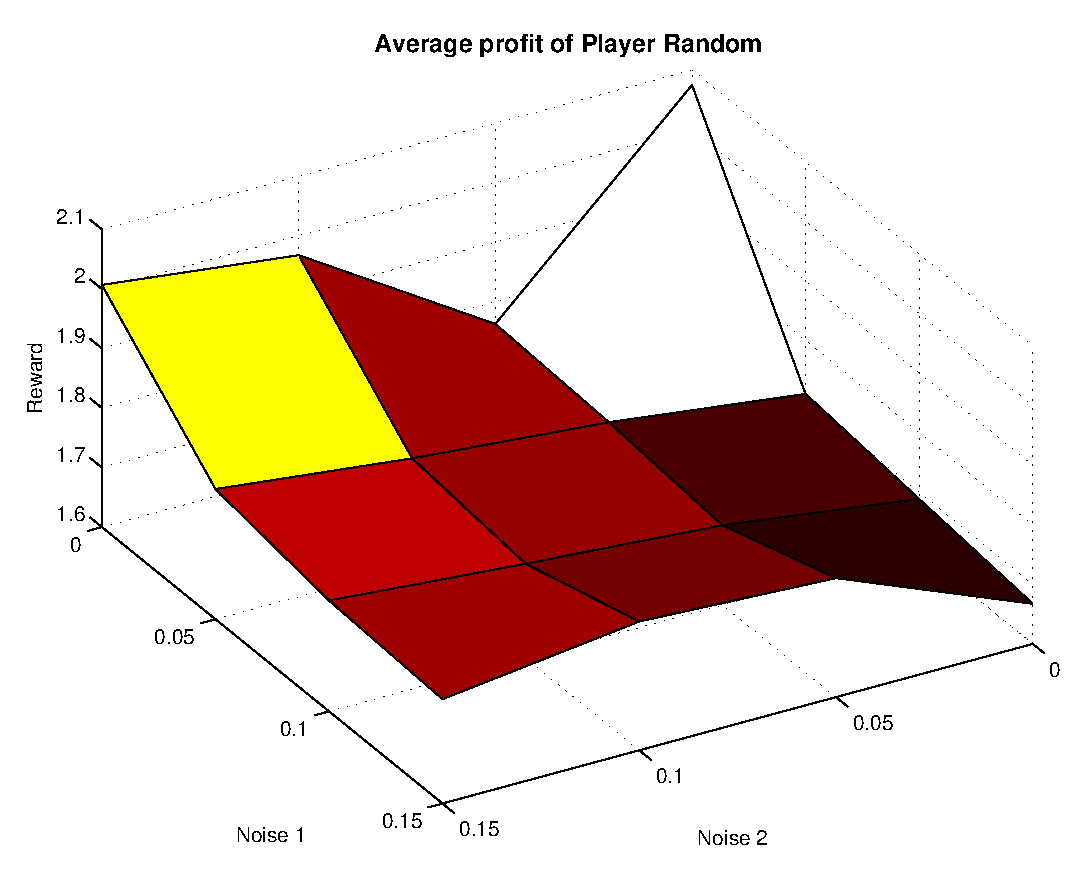
\includegraphics[width=\textwidth]{pics/simulation1/Reward_vs_Noise_of_Player_Random}
\end{minipage}
\hfill
\begin{minipage}[hbt]{0.3\textwidth}
	\centering
	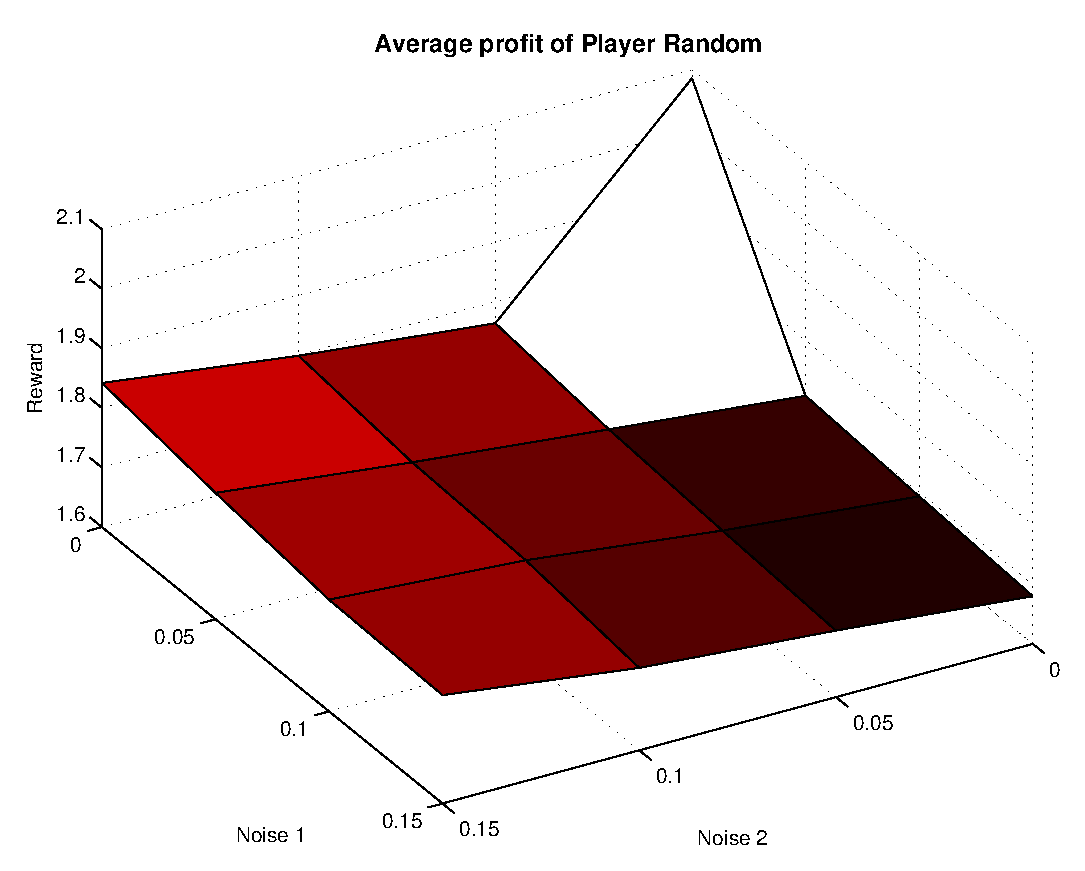
\includegraphics[width=\textwidth]{pics/simulation2/Reward_vs_Noise_of_Player_Random}
\end{minipage}

\end{figure}

The player does not get influenced that much by noise. There is a strange peak at zero noise, we were unable to find out why. If the noise makes his moves appear a little more cooperate there is a slight increase in performance, most likely due to more cooperative reactions from \verb0TFT0 mutants.

\subsubsection{Tit for Tat}
The player's performance is shown in figure~\ref{pic player tit for tat}.\\
\begin{figure}[h]
	\caption{Reward plot of TFT}
	\label{pic player tit for tat}
\begin{minipage}[hbt]{0.65\textwidth}
	\centering
	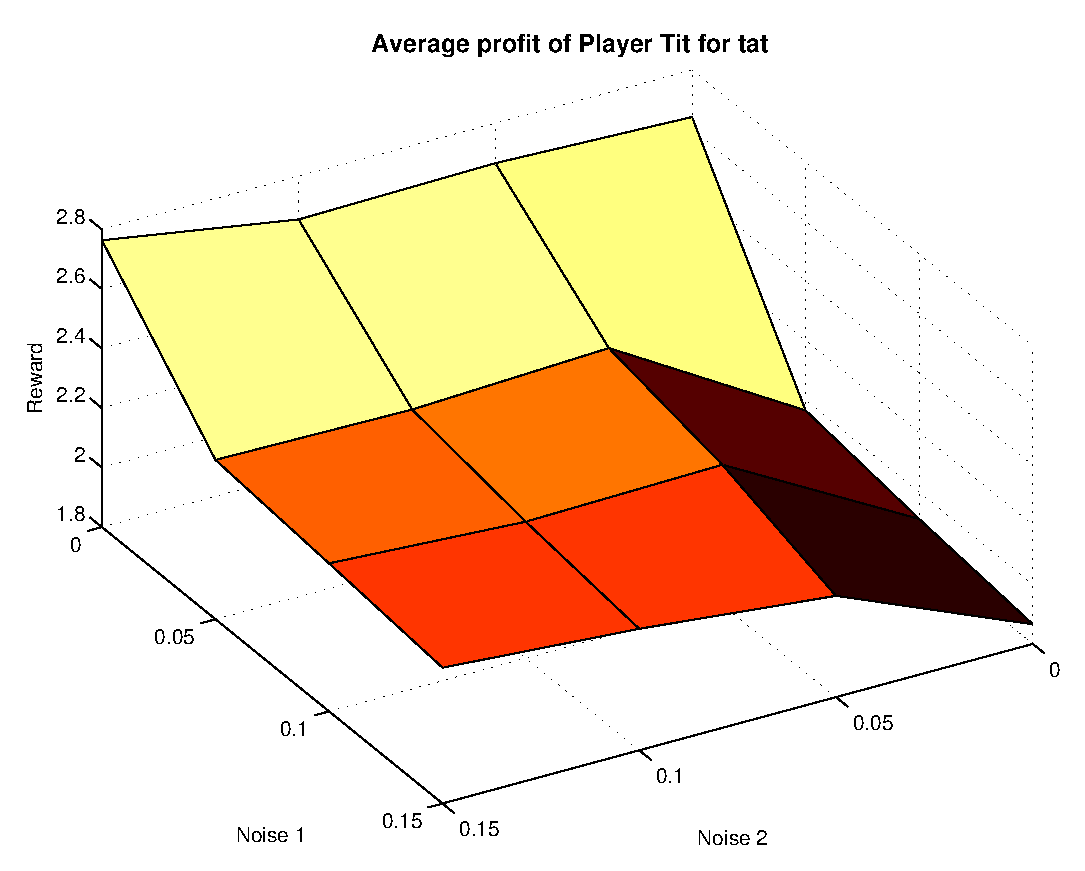
\includegraphics[width=\textwidth]{pics/simulation1/Reward_vs_Noise_of_Player_Tit_for_tat}
\end{minipage}
\hfill
\begin{minipage}[hbt]{0.3\textwidth}
	\centering
	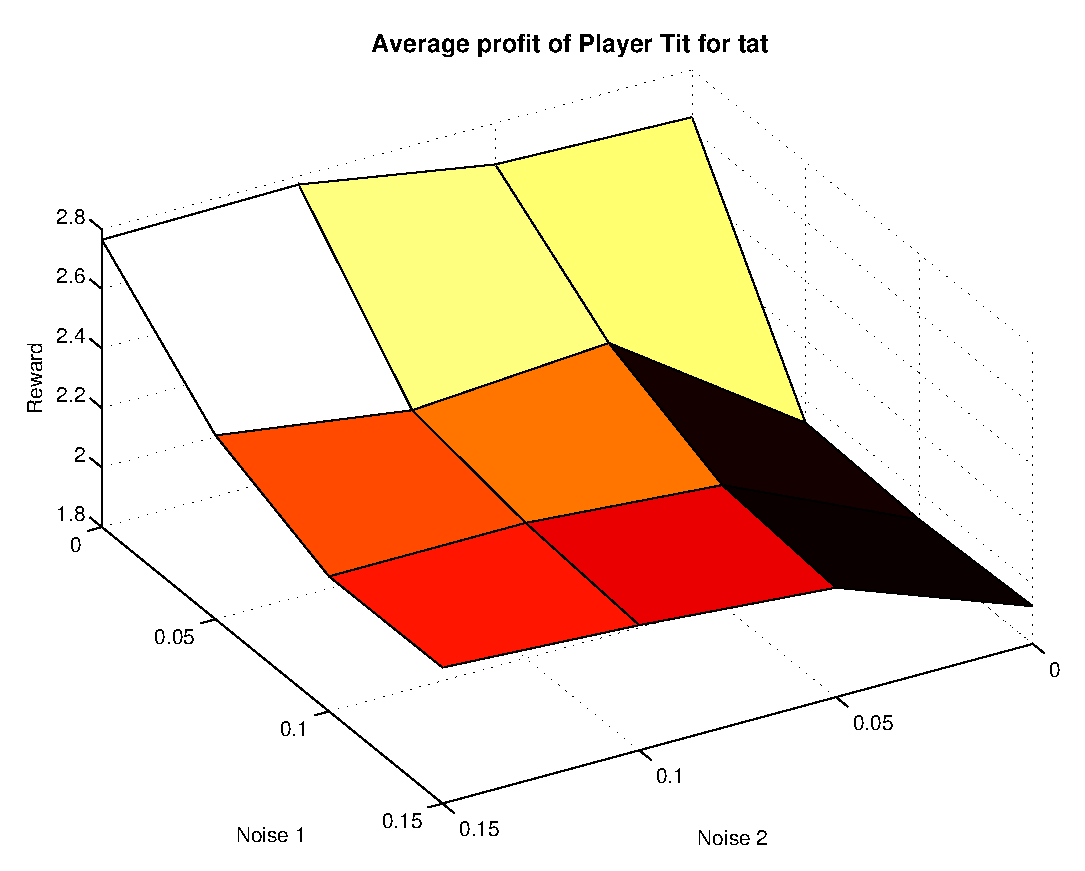
\includegraphics[width=\textwidth]{pics/simulation2/Reward_vs_Noise_of_Player_Tit_for_tat}
\end{minipage}

\end{figure}

\verb0TFT0 is a rather strong player. He won Axelrod's Tournaments, which were without noise. For noise$1$ equals to zero he is one of the strongest of all players. These graphs above show that this player is extremely susceptible to noise$1$. The reason is that with no noise$1$ he will always cooperate with other \verb'TFT' mutants because the first move was cooperative. With noise the first move matters less. There are basically three states he can enter with himself:\\

\renewcommand{\labelitemi}{}

\begin{itemize}
	\item State 1: Mutual cooperation. Performance: $3$
	\item State 2: Alternating defection and cooperation. Performance: $2.5$
	\item State 3: Mutual defection. Performance: $1$
\end{itemize}

 A noise$1$ signal changes the state from state one to state two or state two to state three. Noise$2$ works in the other direction. The two noises are basically transition probabilities. For noise$1$ greater than zero and noise$2$ equal to zero the \verb'TFT' ends up stuck in state three with itself. For equal noises in both directions \verb'TFT' should be $50\%$ of the time in state two and $25\%$ in the states one and three. This would imply the performance: $0.25*3+0.5*2.5+0.25*1=2.25$, as seen in table~\ref{tab:tfttable2}.\\

Table~\ref{tab:tfttable} shows the performance of \verb'TFT' against itself. Because the players in our simulation could only perform mirrored decisions state two was impossible and the actual performance was somewhat lower.\\

\begin{table}[h]
 \begin{center}
\caption{Performance of TFT playing against TFT}\label{tab:tfttable} \vspace{3mm}
\begin{tabular}{|l|c|c|c|c|c|}
\hline
   	& noise2 = 0 & noise2 = 0.05& noise2 = 0.1& noise2 = 0.15 \\
  \hline
  noise1 = 0 	& 3.0000	 &3.0000 	&3.0000	&3.0000 \\
 \hline
  noise1 = 0.05	 & 1.0016	 &2.0127 	&2.3438	&2..4745 \\
 \hline
  noise1 = 0.10 	& 1.0018	 &1.6184 	&1.9847	&2.1967 \\
 \hline
  noise1 = 0.15 	& 1.0011	 &1.5170 	&1.7666	&2.0086 \\
 \hline
\end{tabular}
 \end{center}


\end{table}

\begin{table}[h]
 \begin{center}
\caption{Cooperation of TFT depending on the noise}\label{tab:tfttable2}  \vspace{3mm}
\begin{tabular}{|l|c|c|c|c|c|}
\hline
   	& noise2 = 0 & noise2 = 0.05& noise2 = 0.1& noise2 = 0.15 \\
  \hline
  noise1 = 0 	& 0.8075	 &0.8247 	&0.8351	&0.8917 \\
 \hline
  noise1 = 0.05	 & 0.3958	&    0.5967&    0.6192 &   0.6516 \\
 \hline
  noise1 = 0.10 	& 0.3418 &   0.5127 &   0.5428&   0.5866 \\
 \hline
  noise1 = 0.15 	& 0.2886  &  0.4240 &   0.4836  &  0.5297 \\
 \hline
\end{tabular}
 \end{center}
\end{table}

Already at noise$1=0.05$ the number of cooperative moves \verb'TFT' performs drops from $40\%$ to $80\%$. At higher noise$2$ with no noise$1$ the number of defections performed by \verb'TFT' halves.\\

Traits of the player:

\renewcommand{\labelitemi}{}

\begin{itemize}
	\item + Responds fast
	\item + Not exploitable
	\item + Forgiving
	\item - Only accepts an apology, but does not initiate it himself, so he can stuck in mutual defections!
\end{itemize}
\renewcommand{\labelitemi}{$\bullet$}

\subsubsection{Friedmann}
The player's performance is shown in figure~\ref{pic player friedmann}.\\
\begin{figure}[h]
	\caption{Reward plot of FRI}
	\label{pic player friedmann}
\begin{minipage}[hbt]{0.65\textwidth}
	\centering
	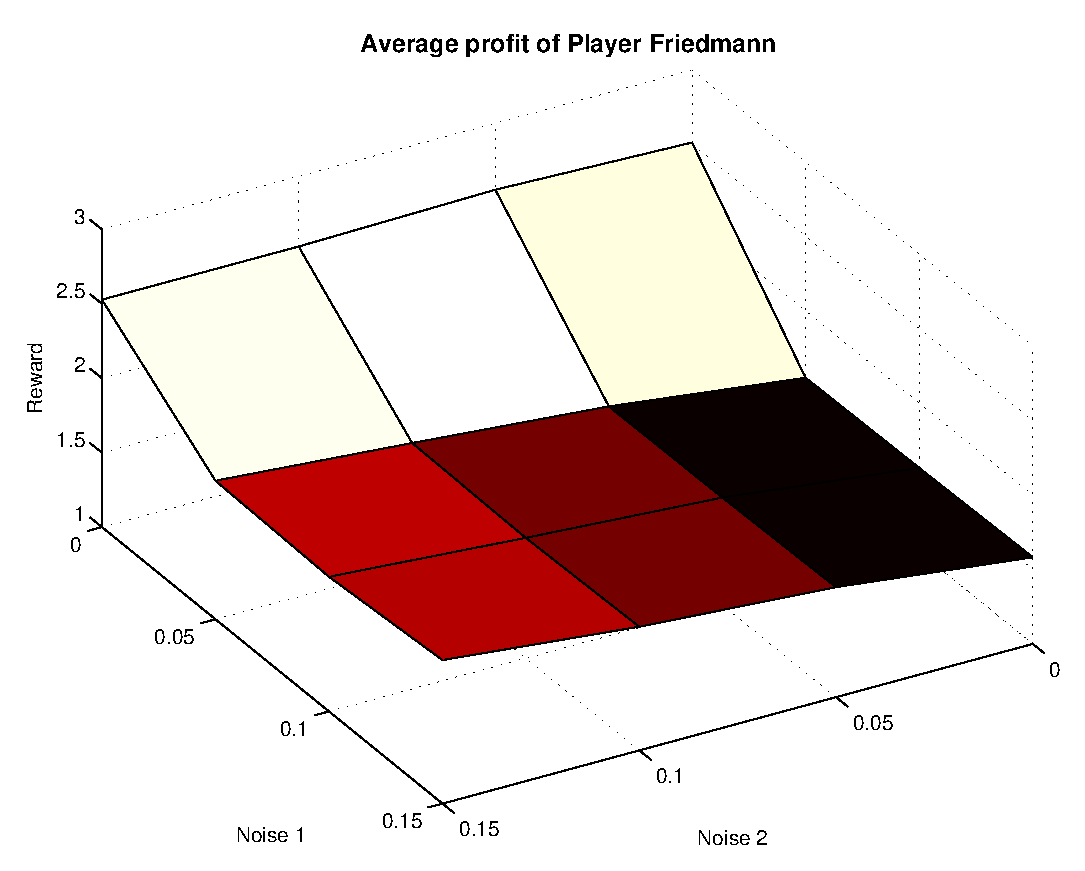
\includegraphics[width=\textwidth]{pics/simulation1/Reward_vs_Noise_of_Player_Friedmann}
\end{minipage}
\hfill
\begin{minipage}[hbt]{0.3\textwidth}
	\centering
	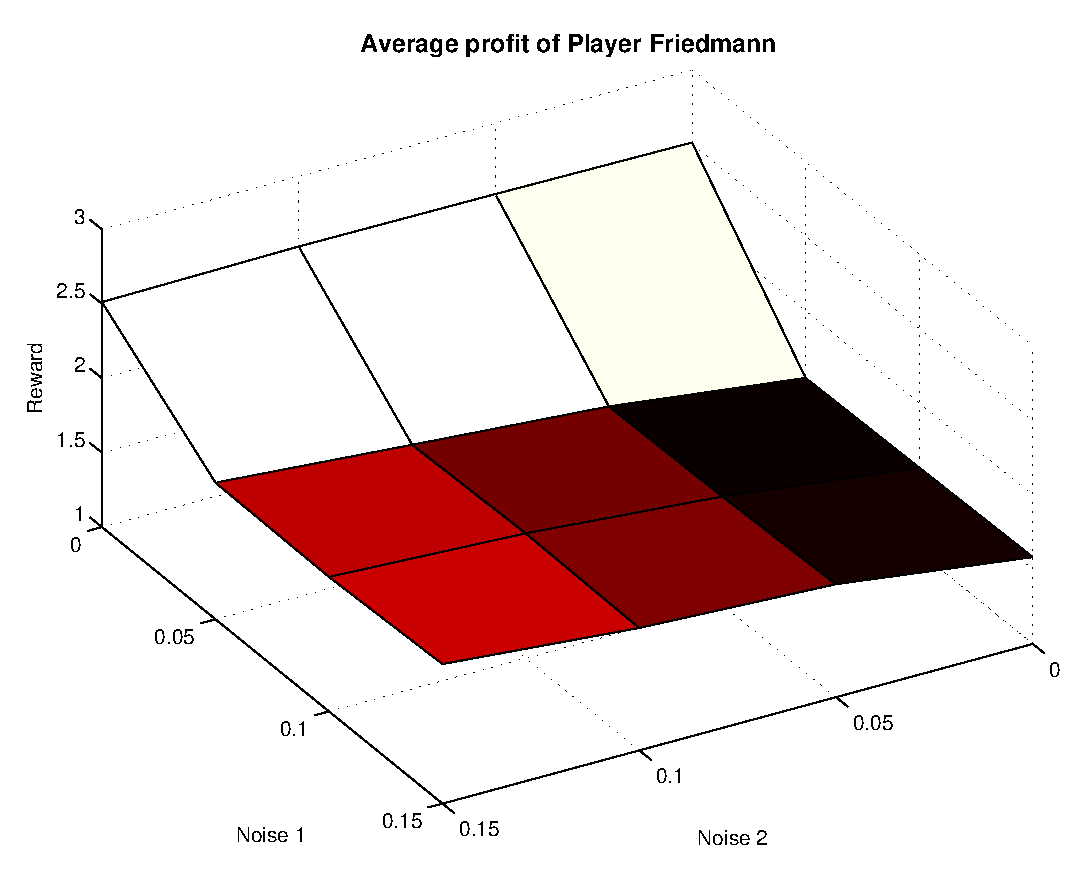
\includegraphics[width=\textwidth]{pics/simulation2/Reward_vs_Noise_of_Player_Friedmann}
\end{minipage}

\end{figure}

In the case of perfect information this player can profit from mutual cooperation with many players. In this case he performs well. However for any noise1 greater than zero the player will receive a rejection at some point and therefore act like the player \verb0DEF0 most of the time. \verb0FRI0 generally tries to retaliate so hard on a rejection that the other player will not even attempt one rejection. However \verb0FRI0 cannot capitalise on this deterrent effect, because the moment the opponent realises it is already too late and he cannot know it in advance.\\

\begin{table}[h]
 \begin{center}
\caption{Cooperation of FRI dependant on the noise} \vspace{3mm}
\begin{tabular}{|l|c|c|c|c|c|}
\hline
   	& noise2 = 0 & noise2 = 0.05& noise2 = 0.1& noise2 = 0.15 \\
  \hline
  noise1 = 0 	& 0.6002&    0.6000&    0.6000 &   0.6000 \\
 \hline
  noise1 = 0.05	 & 0.0004&    0.0001 &   0.0001  &  0.0001 \\
 \hline
  noise1 = 0.10 	& 0.0001  &  0.0001&    0.0001 &   0.00016 \\
 \hline
  noise1 = 0.15 	& 0.0001  &  0.0001  &  0.0001  &  0.0001 \\
 \hline
\end{tabular}
 \end{center}
\end{table}

As soon as noise1 is greater than zero the number of cooperative moves goes to zero. But already at zero noise \verb0FRI0 only has 60\% cooperative moves, while \verb0TFT0 has 80\%.\\


Traits of the player:

\renewcommand{\labelitemi}{}

\begin{itemize}
	\item + Stays in mutual cooperation with friendly players when noise1 is zero
	\item - Completely breaks down with noise1 greater than zero
\end{itemize}
\renewcommand{\labelitemi}{$\bullet$}

\subsubsection{Pavlov}
The player's performance is shown in figure~\ref{pic player pavlov}.\\
\begin{figure}[h]
	\caption{Reward plot of PAV}
	\label{pic player pavlov}
\begin{minipage}[hbt]{0.65\textwidth}
	\centering
	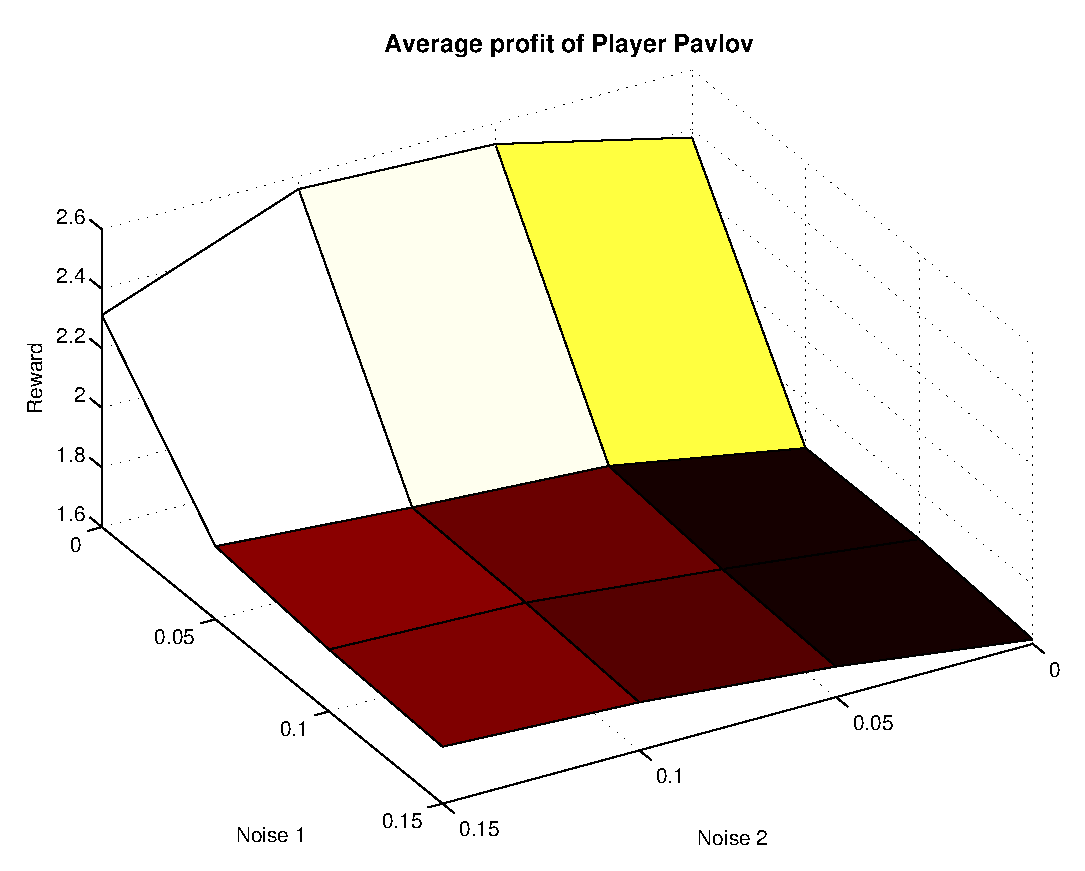
\includegraphics[width=\textwidth]{pics/simulation1/Reward_vs_Noise_of_Player_Pavlov}
\end{minipage}
\hfill
\begin{minipage}[hbt]{0.3\textwidth}
	\centering
	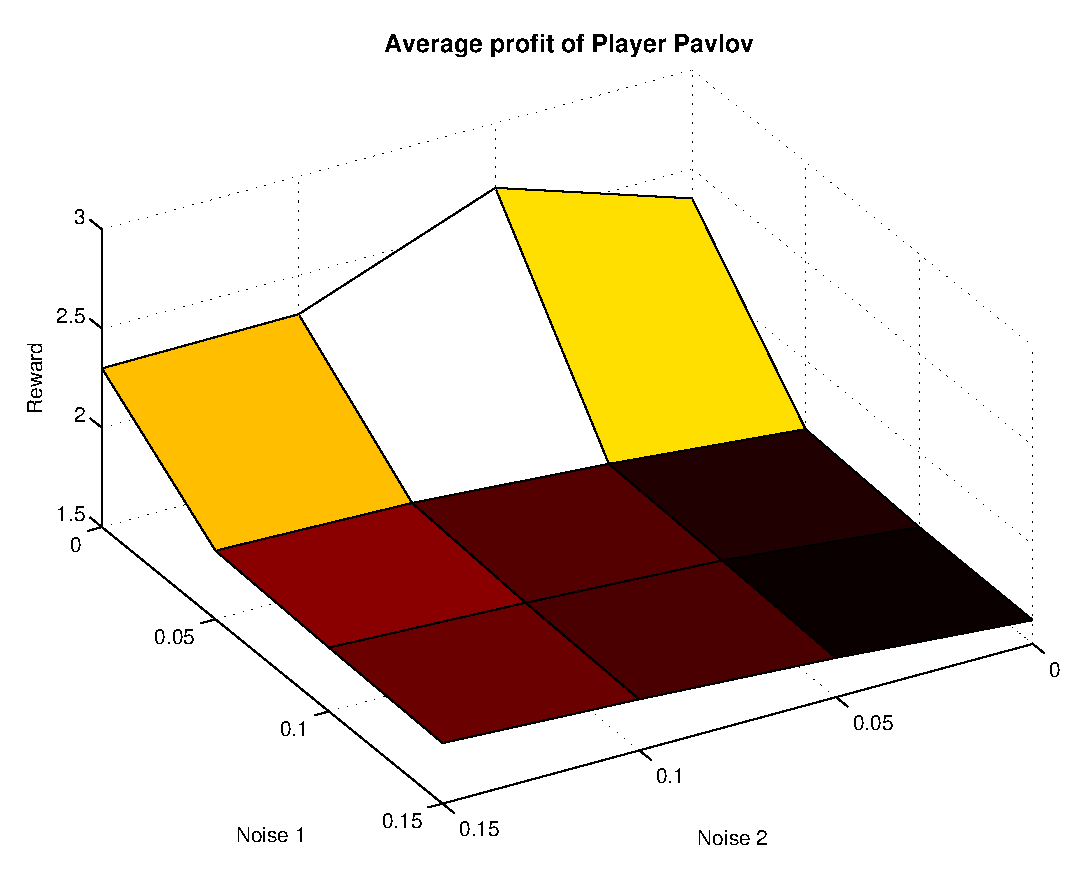
\includegraphics[width=\textwidth]{pics/simulation2/Reward_vs_Noise_of_Player_Pavlov}
\end{minipage}

\end{figure}

\verb0PAV0 performs rather well without noise1. If noise1 is greater then zero, some players realise that defections against \verb0PAV0 work as well as cooperations. Pure defect against \verb0PAV0 results in the rewards 5 1 5 1 5 1 $\ldots$ for the opponent, while pure cooperation results in 3 3 3 3 $\ldots$, given \verb0PAV0 is cooperative when the opponent started playing random. With zero noise the opponent gets an average reward of 3 for cooperation and defection but with noise the performance of cooperation decreases (because \verb0PAV0 retaliates). Players that largely start to defect against \verb0PAV0 are:  \verb0FRI0, \verb0TFAT0, \verb0CDO0, \verb0LCDO0 and \verb0SSW0.

\begin{table}[h]
 \begin{center}
\caption{Cooperation of PAV depending on the noise} \vspace{3mm}
\begin{tabular}{|l|c|c|c|c|c|}
\hline
   	& noise2 = 0 & noise2 = 0.05& noise2 = 0.1& noise2 = 0.15 \\
  \hline
  noise1 = 0 	&     0.8239 &   0.8488&    0.8541&    0.8037 \\
 \hline
  noise1 = 0.05	 &   0.4885  &  0.5433 &   0.5697  &  0.5860 \\
 \hline
  noise1 = 0.10 	& 0.4939  &  0.5211 &   0.5338 &   0.5455 \\
 \hline
  noise1 = 0.15 	& 0.5063    &0.5187  &  0.5251 &   0.5319 \\
 \hline
\end{tabular}
 \end{center}
\end{table}

Without noise1 the number of cooperative moves is around 80\% while it is around 50\% with noise1. It is interesting that with noise2 but no noise1 Pavlov is less cooperative than \verb0TFT0.\\


Traits of the player:

\renewcommand{\labelitemi}{}
\begin{itemize}
	\item + Forgives fast
	\item + Initializes cooperation out of mutual defection
	\item + Not exploitable without noise
	\item - Too many cooperative moves against defecting players
	\item - Not retaliating (pure defect and pure cooperation perform equally well)
\end{itemize}
\renewcommand{\labelitemi}{$\bullet$}

\subsubsection{Tit for 2 Tat}
The player's performance is shown in figure~\ref{pic player tf2t}.\\
\begin{figure}[h]
	\caption{Reward plot of TF2T}
	\label{pic player tf2t}
\begin{minipage}[hbt]{0.65\textwidth}
	\centering
	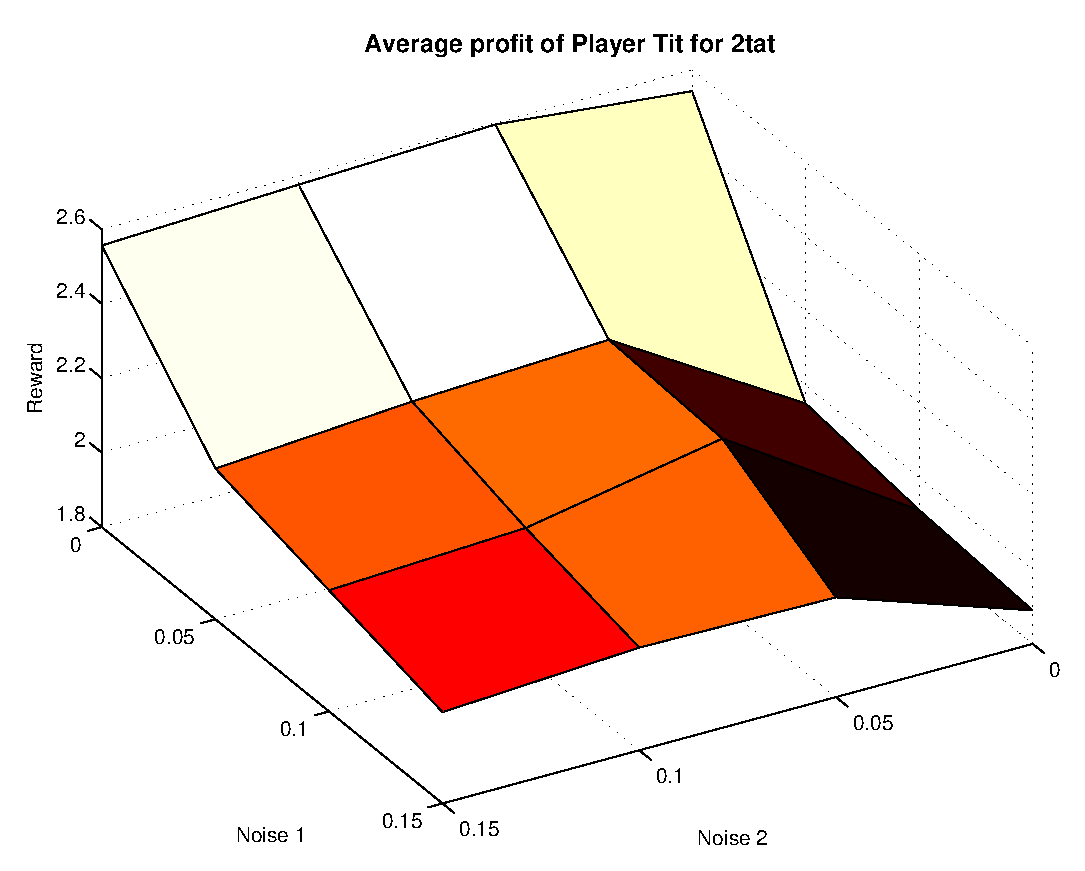
\includegraphics[width=\textwidth]{pics/simulation1/Reward_vs_Noise_of_Player_Tit_for_2tat}
\end{minipage}
\hfill
\begin{minipage}[hbt]{0.3\textwidth}
	\centering
	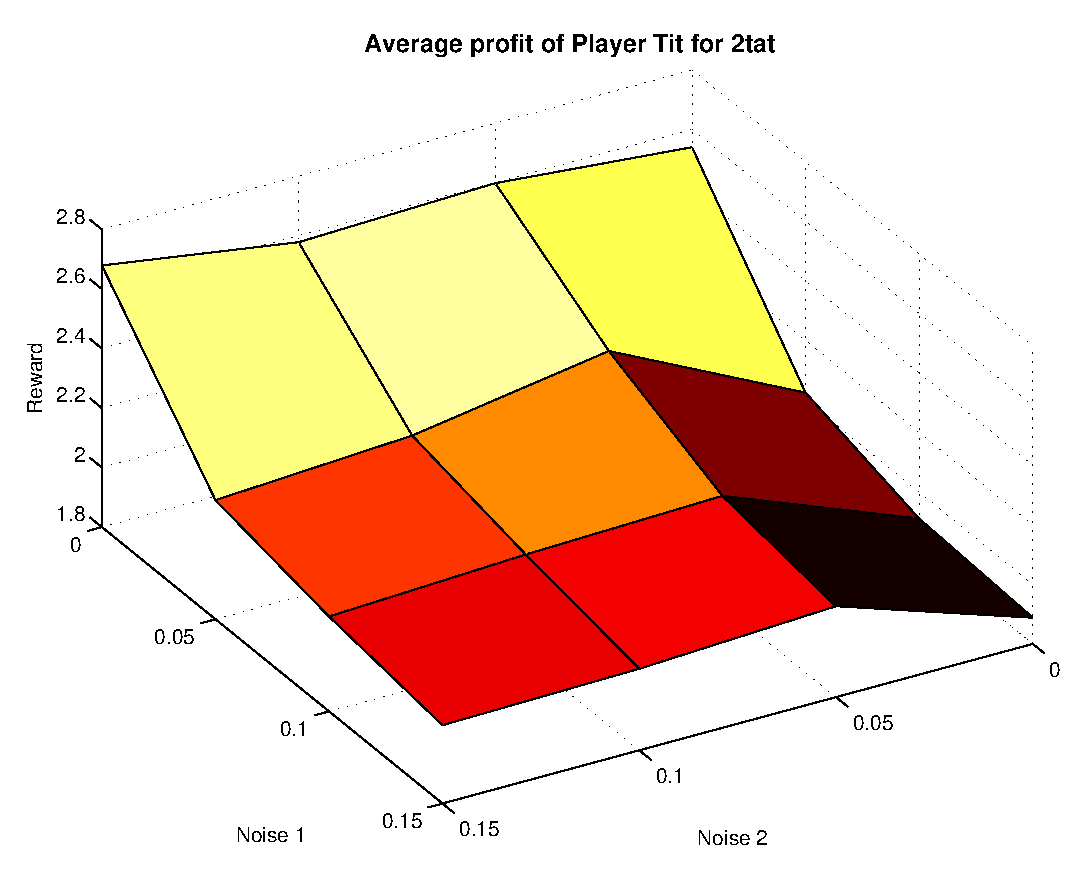
\includegraphics[width=\textwidth]{pics/simulation2/Reward_vs_Noise_of_Player_Tit_for_2tat}
\end{minipage}

\end{figure}

As a \verb'TFT' mutant it has a similar performance. The difference is that this player is more forgiving. The bad thing is that this makes him exploitable. The better thing is that it is more robust to noise1 as it does not react to single defections. The player still ends up in mutual defections with itself if noise2 is zero and noise1 greater than zero, but for both noises greater than zero the player plays much stronger against itself. At zero noise the performance of \verb0TF2T0 is worse than the one of \verb0TFT0, but with noise1 their performances are similar. The effect that players like \verb0EVO0 will exploit \verb0TF2T0 seems to balance out with the better resistance to noise.\\

\begin{table}[h]
 \begin{center}
\caption{Cooperation of TF2T depending on the noise} \vspace{3mm}
\begin{tabular}{|l|c|c|c|c|c|}
\hline
   	& noise2 = 0 & noise2 = 0.05& noise2 = 0.1& noise2 = 0.15 \\
  \hline
  noise1 = 0 	&        0.8271&    0.8796 &   0.8880  & 0.8947 \\
 \hline
  noise1 = 0.05	 &       0.5366  &  0.7450  &  0.7712 &   0.7926 \\
 \hline
  noise1 = 0.10 	&    0.5132 &   0.7349  &  0.7375&   0.7622 \\
 \hline
  noise1 = 0.15 	&     0.4864 &   0.6503 &   0.6977   & 0.72749 \\
 \hline
\end{tabular}
 \end{center}
\end{table}

The cooperation stays much higher than for \verb0TFT0 especially if noise2 also is not equal to zero.\\

Traits different to \verb0TFT0:

\renewcommand{\labelitemi}{}
\begin{itemize}
	\item + More Forgiving
	\item - More Exploitable
\end{itemize}
\renewcommand{\labelitemi}{$\bullet$}
 
\subsubsection{Joss}
The player's performance is shown in figure~\ref{pic player joss}.\\
\begin{figure}[h]
	\caption{Reward plot of JOSS}
	\label{pic player joss}
\begin{minipage}[hbt]{0.65\textwidth}
	\centering
	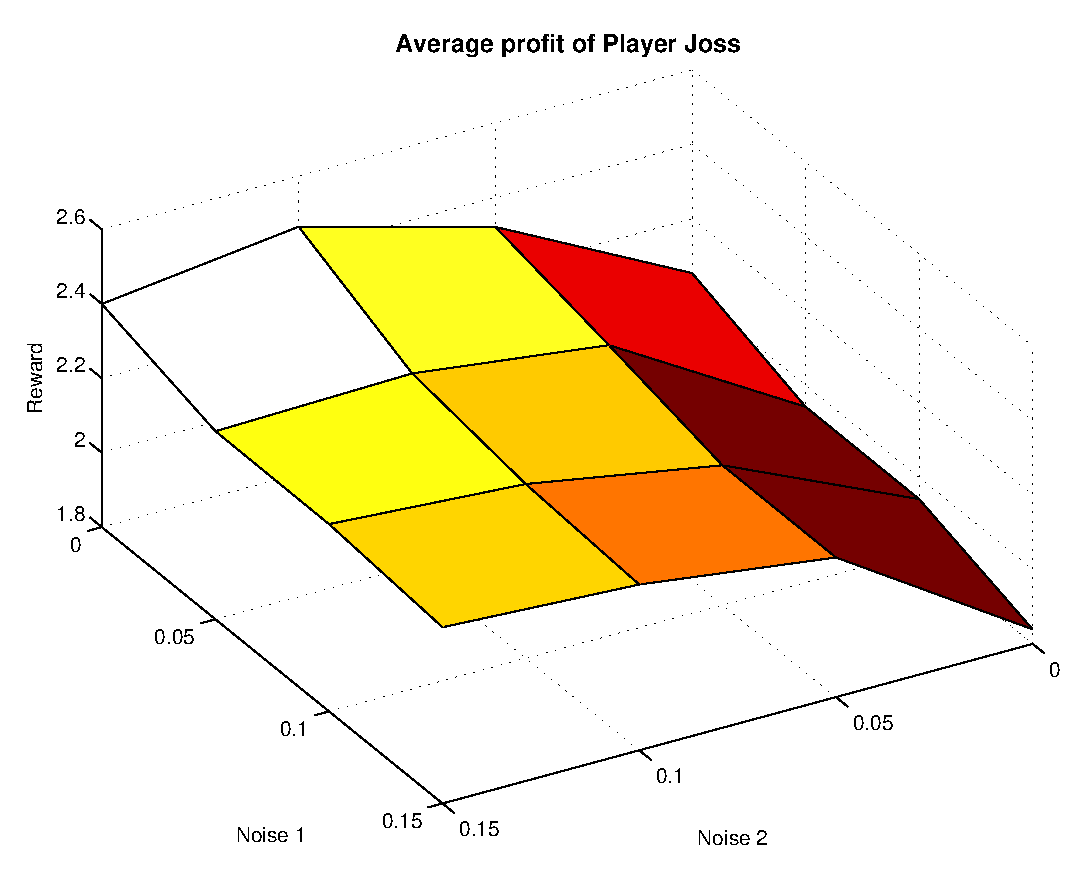
\includegraphics[width=\textwidth]{pics/simulation1/Reward_vs_Noise_of_Player_Joss}
\end{minipage}
\hfill
\begin{minipage}[hbt]{0.3\textwidth}
	\centering
	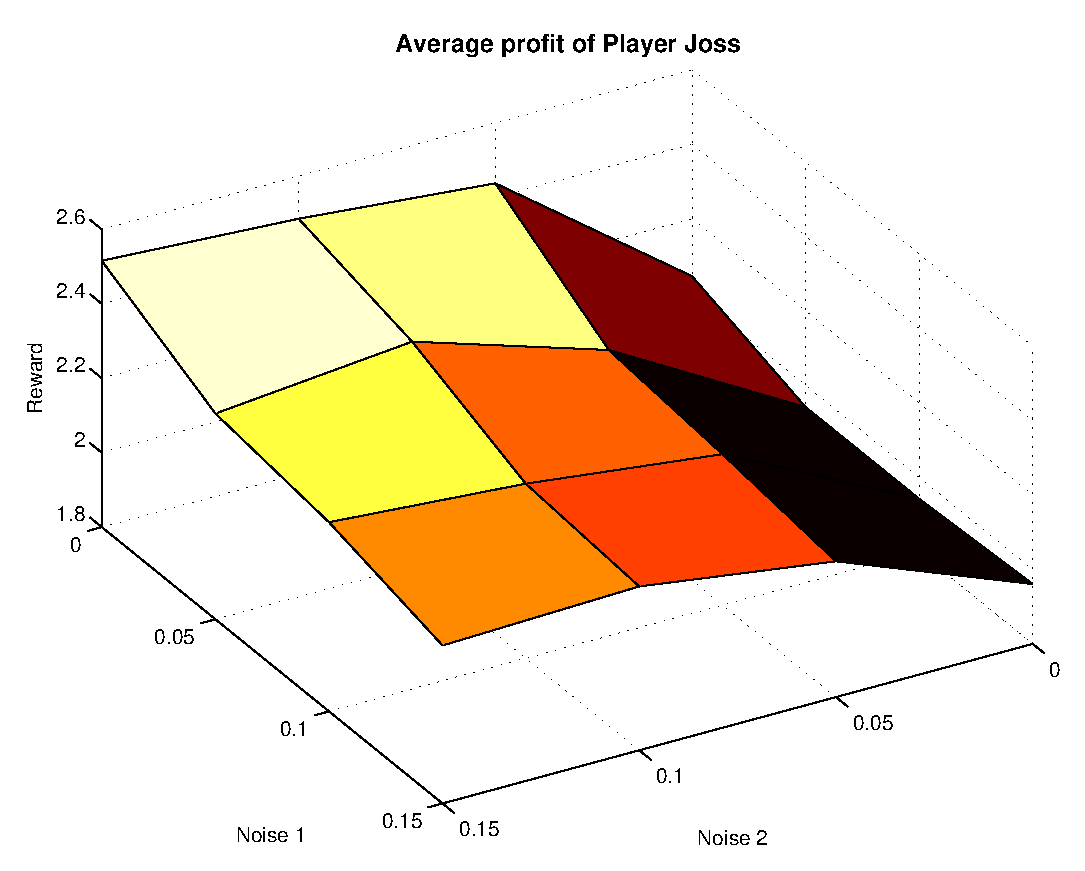
\includegraphics[width=\textwidth]{pics/simulation2/Reward_vs_Noise_of_Player_Joss}
\end{minipage}

\end{figure}

While this is a \verb0TFT0 mutant, its performance dependence on noise looks totally different. The player generally performs poorly. At some noises this player is able to exploit \verb0TF2T0 (noise2 greater than zero and noise1 equal to zero) however most of the time the retaliation of the defections outweighs their gain. \verb0TFT0 is very susceptible to noise1 and Joss makes himself look like under noise1 to his opponent. It is interesting that the performance of this player looks like the performance of \verb0DEF0 just shifted about 0.5 upwards.\\

\begin{table}[h]
 \begin{center}
\caption{Cooperation of JOSS depending on the noise} \vspace{3mm}
\begin{tabular}{|l|c|c|c|c|c|}
\hline
   	& noise2 = 0 & noise2 = 0.05& noise2 = 0.1& noise2 = 0.15 \\
  \hline
  noise1 = 0 	&            0.3983  &  0.5300  &  0.6102  &  0.6172 \\
 \hline
  noise1 = 0.05	 &          0.3983 &   0.5300  &  0.6102 &  0.6172 \\
 \hline
  noise1 = 0.10 	&        0.2968  &  0.4026  &  0.4625    &0.5006 \\
 \hline
  noise1 = 0.15 	&     0.2404    &0.3720 &   0.4225  &  0.4591 \\
 \hline
\end{tabular}
 \end{center}
\end{table}

With higher noise2 some cooperation can be achieved, but generally the player is mostly defecting.\\

Traits different to \verb0TFT0:

\renewcommand{\labelitemi}{}
\begin{itemize}
	\item - initates defections
\end{itemize}
\renewcommand{\labelitemi}{$\bullet$}

\subsubsection{Diekmann}
The player's performance is shown in figure~\ref{pic player diekmann}.\\
\begin{figure}[h]
	\caption{Reward plot of DIE}
	\label{pic player diekmann}
\begin{minipage}[hbt]{0.65\textwidth}
	\centering
	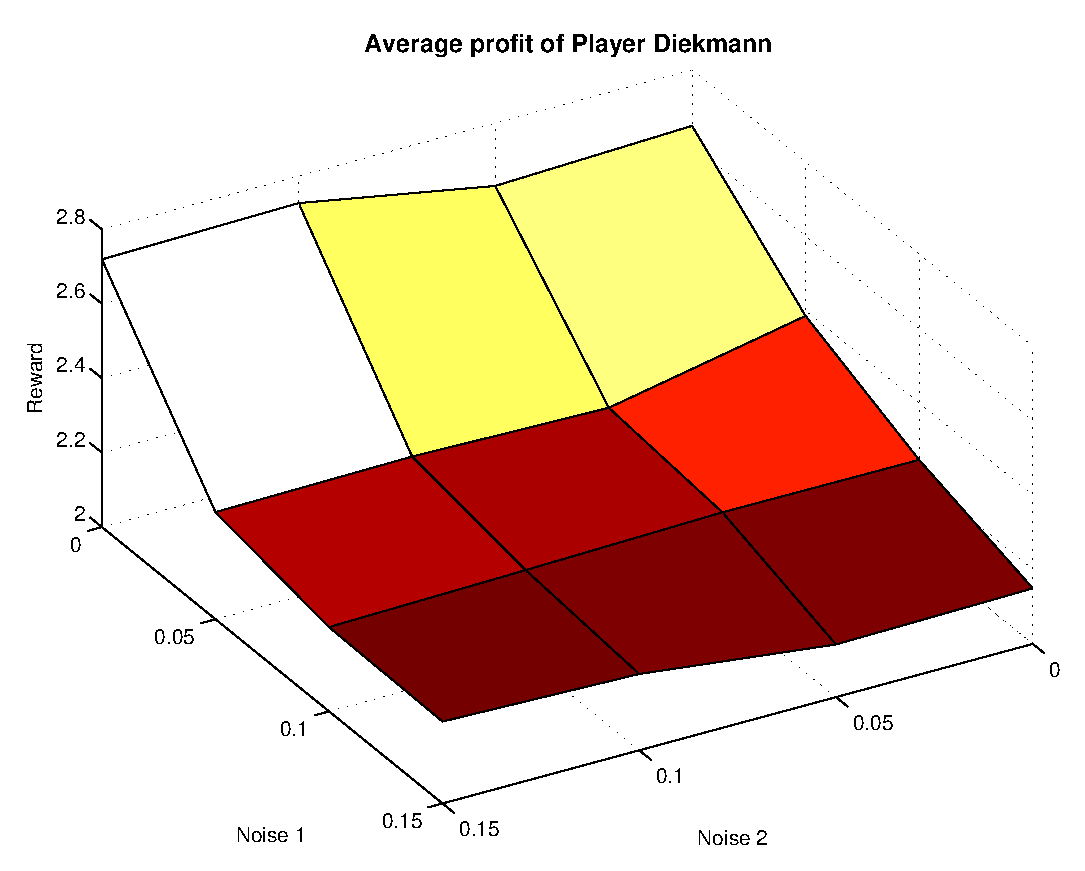
\includegraphics[width=\textwidth]{pics/simulation1/Reward_vs_Noise_of_Player_Diekmann}
\end{minipage}
\hfill
\begin{minipage}[hbt]{0.3\textwidth}
	\centering
	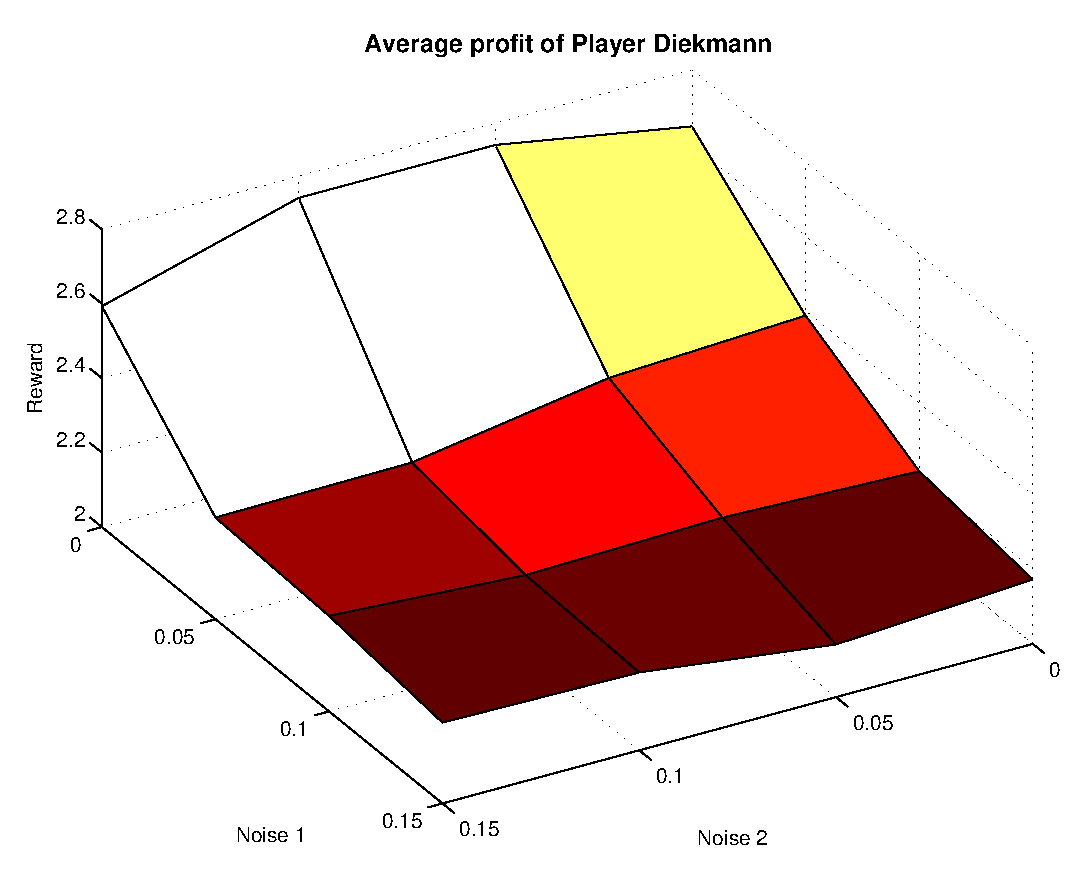
\includegraphics[width=\textwidth]{pics/simulation2/Reward_vs_Noise_of_Player_Diekmann}
\end{minipage}

\end{figure}

This is a \verb0TFT0 mutant, that performs on the same level as \verb0TFT0 at no noise, and is therefore one of the strongest players if there is no noise. While his performance also drops with noise1 the effect is much less severe. For noise1=0.05 and noise2 equal to zero, \verb0TFT0 drops about 0.9, while \verb0DIE0 only drops 0.5. This player actually initiates cooperation and gets not stuck in mutual defection with \verb0TFT0 mutants. The weakness of this player is that he is exploitable by defective moves every 10 moves. However on our simulation we haven't seen a player exploiting this weakness. \verb0EVO0 could exploit it if the period in which the algorithm updates would be a multiple of the period in which \verb0DIE0 inserts cooperative moves.\\

\begin{table}[h]
 \begin{center}
\caption{Cooperation of DIE depending on the noise} \vspace{3mm}
\begin{tabular}{|l|c|c|c|c|c|}
\hline
   	& noise2 = 0 & noise2 = 0.05& noise2 = 0.1& noise2 = 0.15 \\
  \hline
  noise1 = 0 	&               0.8635 &   0.9034   & 0.9113 &  0.8741 \\
 \hline
  noise1 = 0.05	 &            0.7157 &   0.7263  &  0.7200  &  0.7359 \\
 \hline
  noise1 = 0.10 	&           0.6230  &  0.6500  &  0.6655 &   0.6946 \\
 \hline
  noise1 = 0.15 	&   0.5760 &   0.5895  &  0.6283 &   0.6496 \\
 \hline
\end{tabular}
 \end{center}
\end{table}

The cooperation drops not nearly as much with the noise as this is the case for \verb0TFT0, he even is much more cooperative at no noise. At low noise2 values he is more cooperative than \verb0TF2T0, but when both noises get high \verb0TF2T0 is more cooperative.\\

Traits different to \verb0TFT0:

\renewcommand{\labelitemi}{}
\begin{itemize}
	\item + initates cooperation
	\item - More Exploitable
\end{itemize}
\renewcommand{\labelitemi}{$\bullet$}
 
\subsubsection{Tit for Average Tat}
The player's performance is shown in figure~\ref{pic player tfat}.\\
\begin{figure}[h]
	\caption{Reward plot of TFAT}
	\label{pic player tfat}
\begin{minipage}[hbt]{0.65\textwidth}
	\centering
	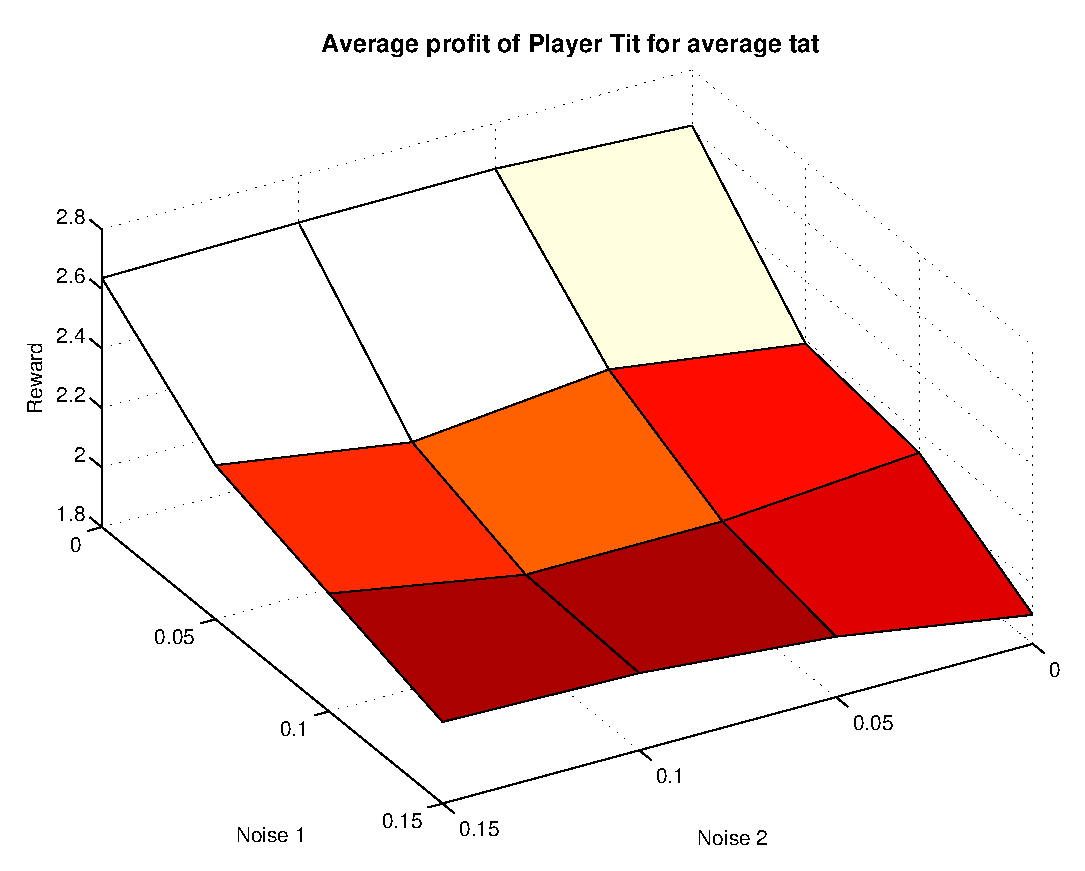
\includegraphics[width=\textwidth]{pics/simulation1/Reward_vs_Noise_of_Player_Tit_for_average_tat}
\end{minipage}
\hfill
\begin{minipage}[hbt]{0.3\textwidth}
	\centering
	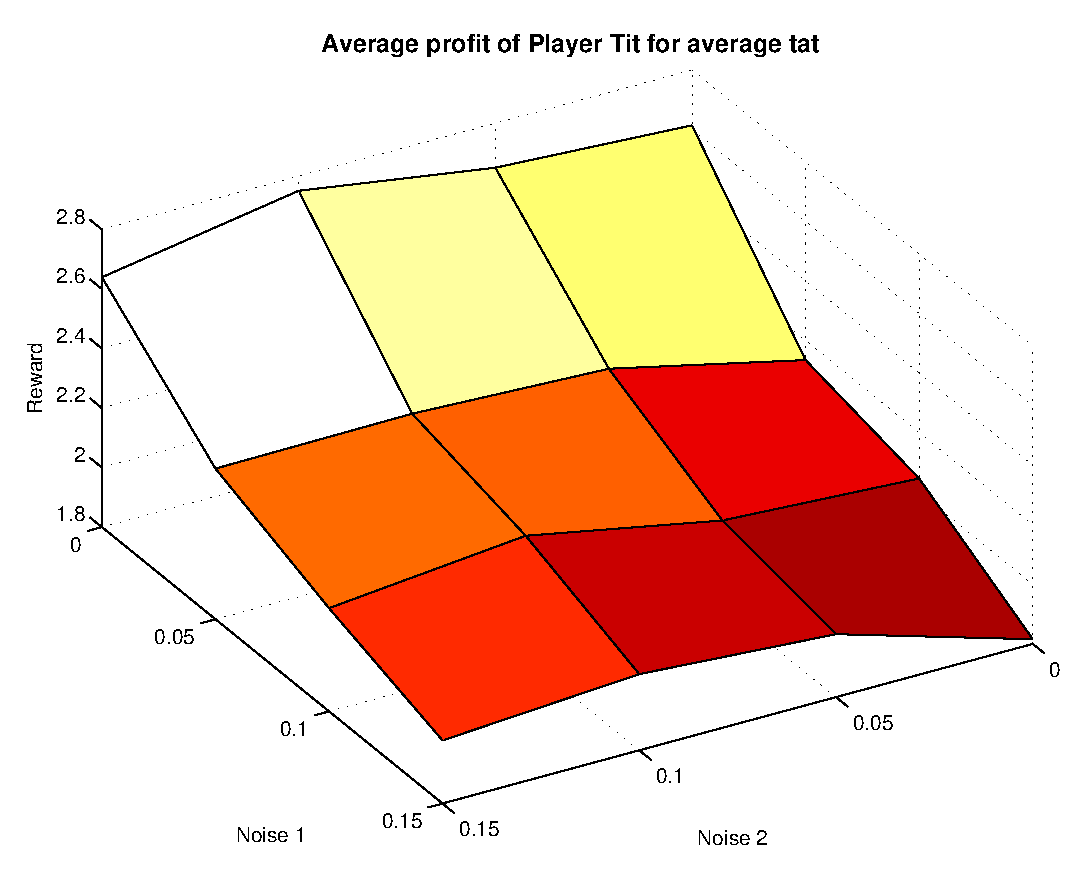
\includegraphics[width=\textwidth]{pics/simulation2/Reward_vs_Noise_of_Player_Tit_for_average_tat}
\end{minipage}

\end{figure}

This \verb0TFT0 mutant looks very similar to \verb0DIE0 and other friendlier \verb0TFT0 mutants. The fact that it reacts to the players average move during the last turns allows him to ignore some of the noise. The problem is that if mutual defection appears it is just as hard to get out of it as it was to get into it. Maybe this players performance would have decreased if the simulation was run even longer. In general this player performs about as well as \verb0RTFT0 and a little bit worse than \verb0DIE0. Theoretically this player is exploitable. \\

\begin{table}[h]
 \begin{center}
\caption{Cooperation of TFAT depending on the noise} \vspace{3mm}
\begin{tabular}{|l|c|c|c|c|c|}
\hline
   	& noise2 = 0 & noise2 = 0.05& noise2 = 0.1& noise2 = 0.15 \\
  \hline
  noise1 = 0 	&    0.8056  &  0.8404  &  0.8456  &  0.8547 \\
 \hline
  noise1 = 0.05	 &     0.5316  &  0.6170 &   0.6140   & 0.6863 \\
 \hline
  noise1 = 0.10 	&    0.4712  &  0.4860  &  0.5100  &  0.5985 \\
 \hline
  noise1 = 0.15 	&       0.3419  &  0.4134 &   0.4660 &   0.5098 \\
 \hline
\end{tabular}
 \end{center}
\end{table}

The cooperation drops surprisingly fast with noise1, but still not as fast as for \verb0TFT0. The number of cooperative moves is still more similar to \verb0TFT0 than \verb0DIE0. This is surprising, that the performances look so close, while the underlying moves are so different. \verb0DIE0 very nice approach seems to be just as efficient as \verb0TFAT0's more retaliating method. \\

Traits of the player:

\renewcommand{\labelitemi}{}
\begin{itemize}
	\item + ignores single moves
	\item - Exploitable
\end{itemize}
\renewcommand{\labelitemi}{$\bullet$}
 
\subsubsection{Reconciliation Tit for Tat}
The player's performance is shown in figure~\ref{pic player rtft}.\\
\begin{figure}[h]
	\caption{Reward plot of RTFT}
	\label{pic player rtft}
\begin{minipage}[hbt]{0.65\textwidth}
	\centering
	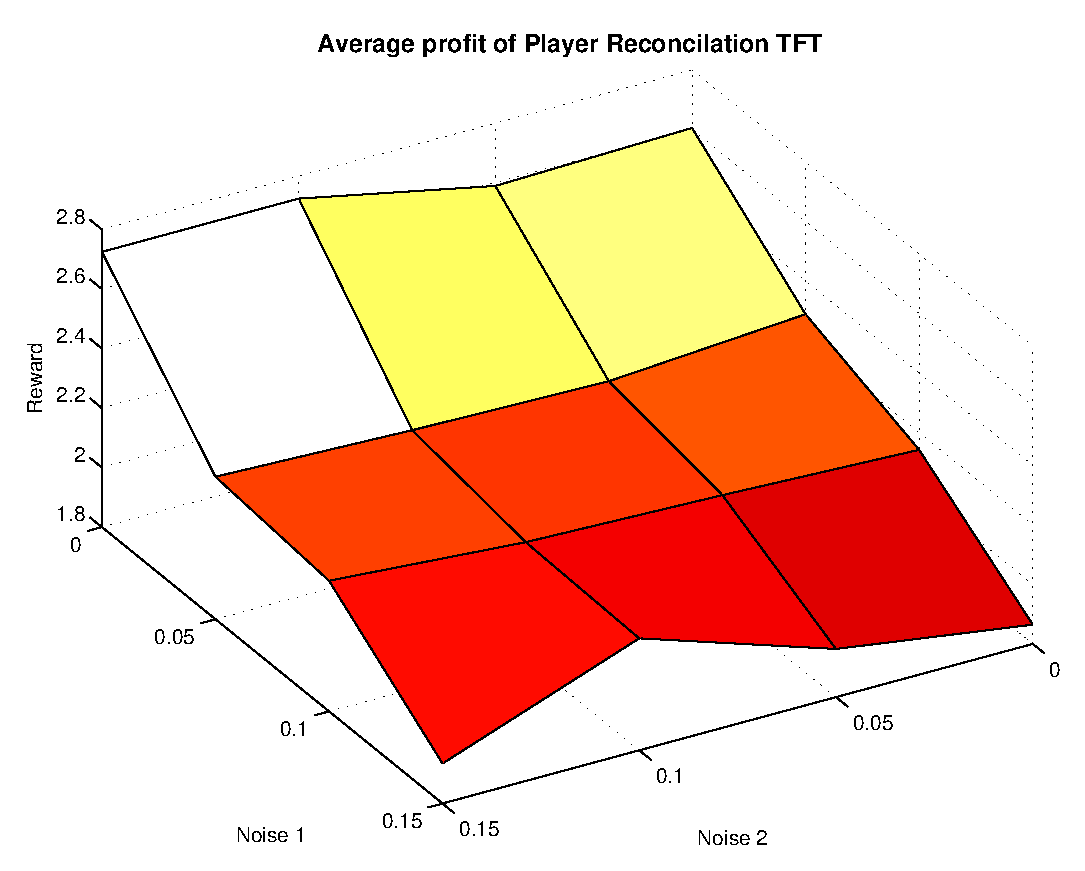
\includegraphics[width=\textwidth]{pics/simulation1/Reward_vs_Noise_of_Player_Reconcilation_TFT}
\end{minipage}
\hfill
\begin{minipage}[hbt]{0.3\textwidth}
	\centering
	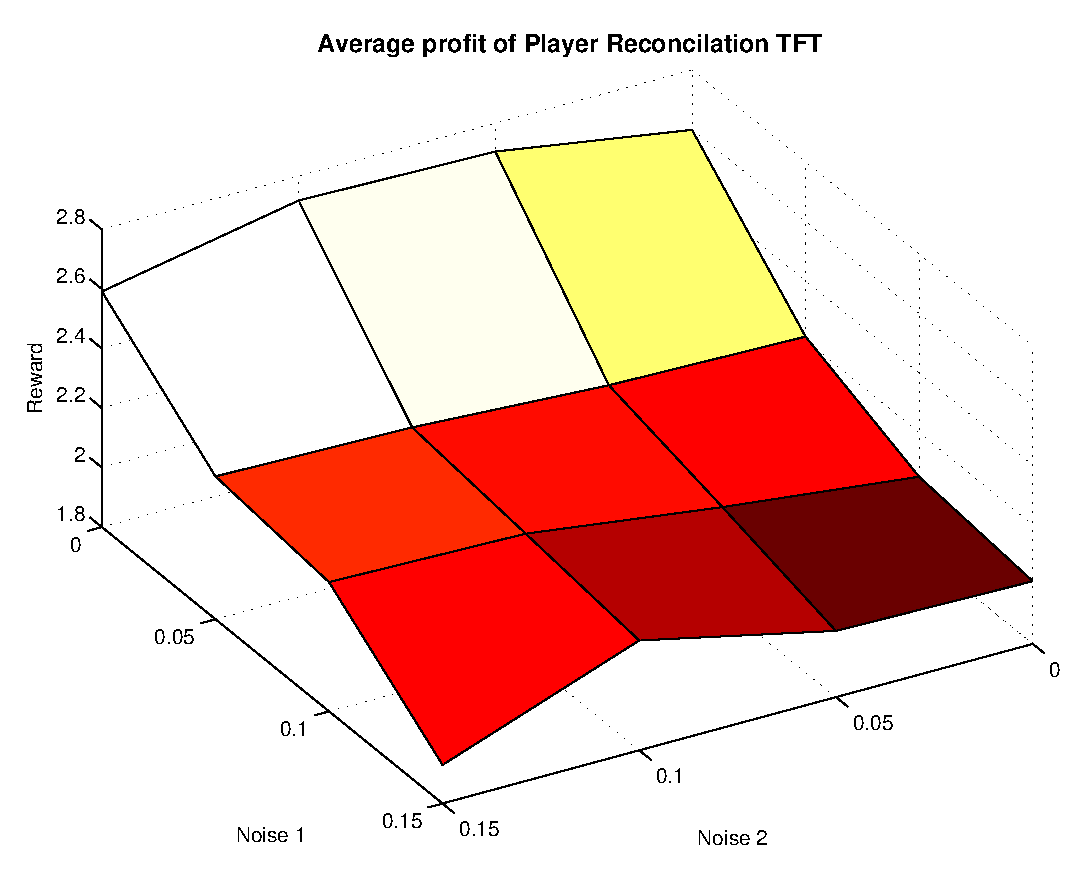
\includegraphics[width=\textwidth]{pics/simulation2/Reward_vs_Noise_of_Player_Reconcilation_TFT}
\end{minipage}

\end{figure}

Like other more forgiving \verb0TFT0 mutants he has similar performance to \verb0TFT0 without noise, and drops less with noise1. The disadvantage of this player is that while it is not exploitable it still performs worse against defective players, when its reconciliation attempts are shut down over and over again.\\

\begin{table}[h]
 \begin{center}
\caption{Cooperation of RTFT depending on the noise} \vspace{3mm}
\begin{tabular}{|l|c|c|c|c|c|}
\hline
   	& noise2 = 0 & noise2 = 0.05& noise2 = 0.1& noise2 = 0.15 \\
  \hline
  noise1 = 0 	&  0.8728  &  0.8972  &  0.9033 &   0.8723 \\
 \hline
  noise1 = 0.05	 &       0.7169 &   0.7218  &  0.7397 &   0.7450 \\
 \hline
  noise1 = 0.10 	&       0.6861 &   0.7010 &   0.7175  &  0.7217 \\
 \hline
  noise1 = 0.15 	&      0.6930 &   0.6955  &  0.7161  &  0.67528 \\
 \hline
\end{tabular}
 \end{center}
\end{table}

The number of cooperations is very high even with high noise1, at noise1=0.15 it's cooperation is higher than that of most \verb0TFT0 mutants. Generally the number of cooperative moves is more similar to \verb0DIE0 than to \verb0TFAT0.\\

Traits different to \verb0TFT0:

\renewcommand{\labelitemi}{}
\begin{itemize}
	\item + Initiates Cooperation
\end{itemize}
\renewcommand{\labelitemi}{$\bullet$}
 
\subsubsection{CDowning and DDowning}
The two players' performance is shown in figure~\ref{pic player cd} (\verb0CDO0) and figure~\ref{pic player dd} (\verb0DDO0).\\
\begin{figure}[h]
	\caption{Reward plot of CDO}
	\label{pic player cd}
\begin{minipage}[hbt]{0.65\textwidth}
	\centering
	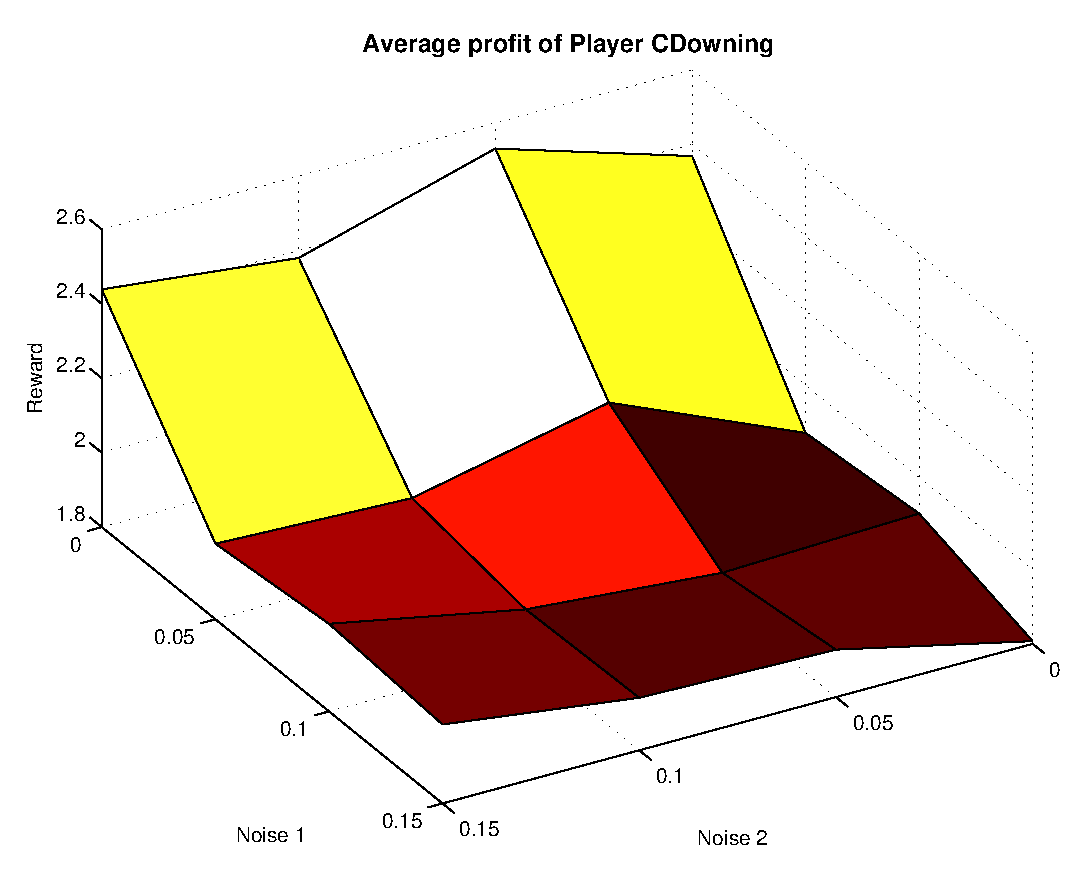
\includegraphics[width=\textwidth]{pics/simulation1/Reward_vs_Noise_of_Player_CDowning}
\end{minipage}
\hfill
\begin{minipage}[hbt]{0.3\textwidth}
	\centering
	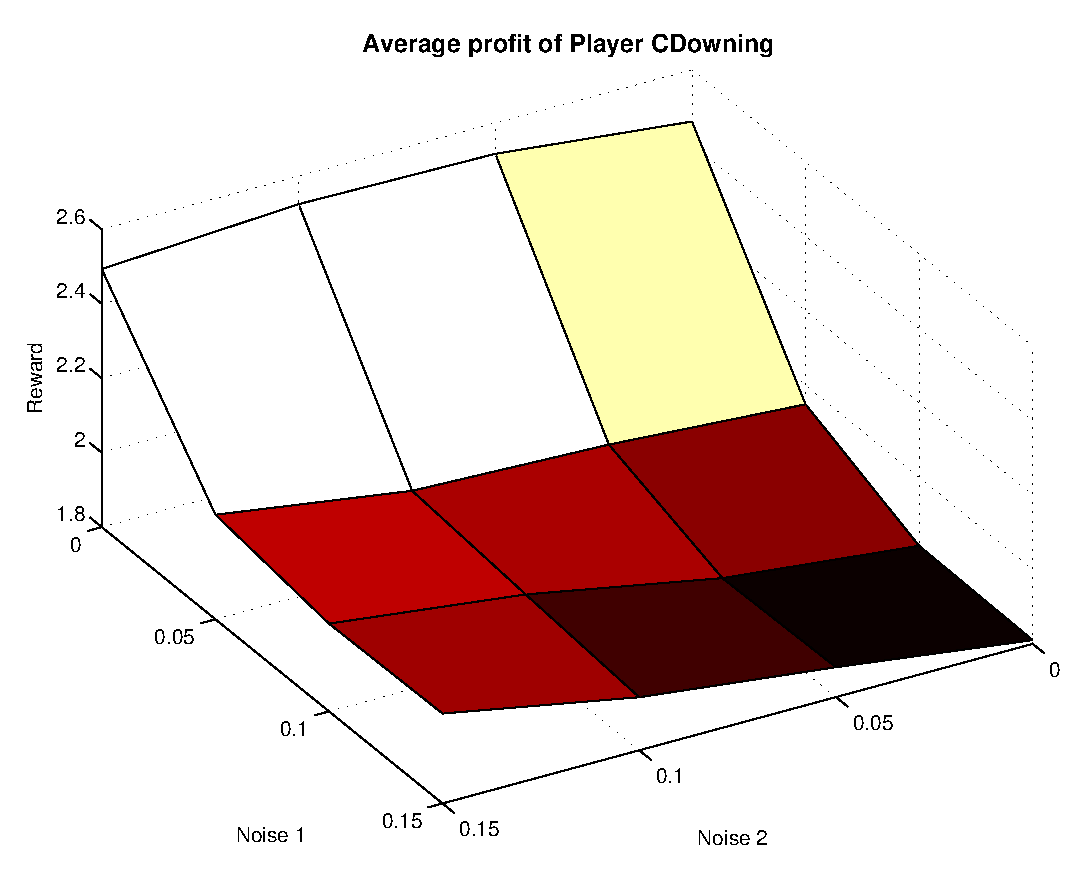
\includegraphics[width=\textwidth]{pics/simulation2/Reward_vs_Noise_of_Player_CDowning}
\end{minipage}

\end{figure}

\begin{figure}[h]
	\caption{Reward plot of DDO}
	\label{pic player dd}
\begin{minipage}[hbt]{0.65\textwidth}
	\centering
	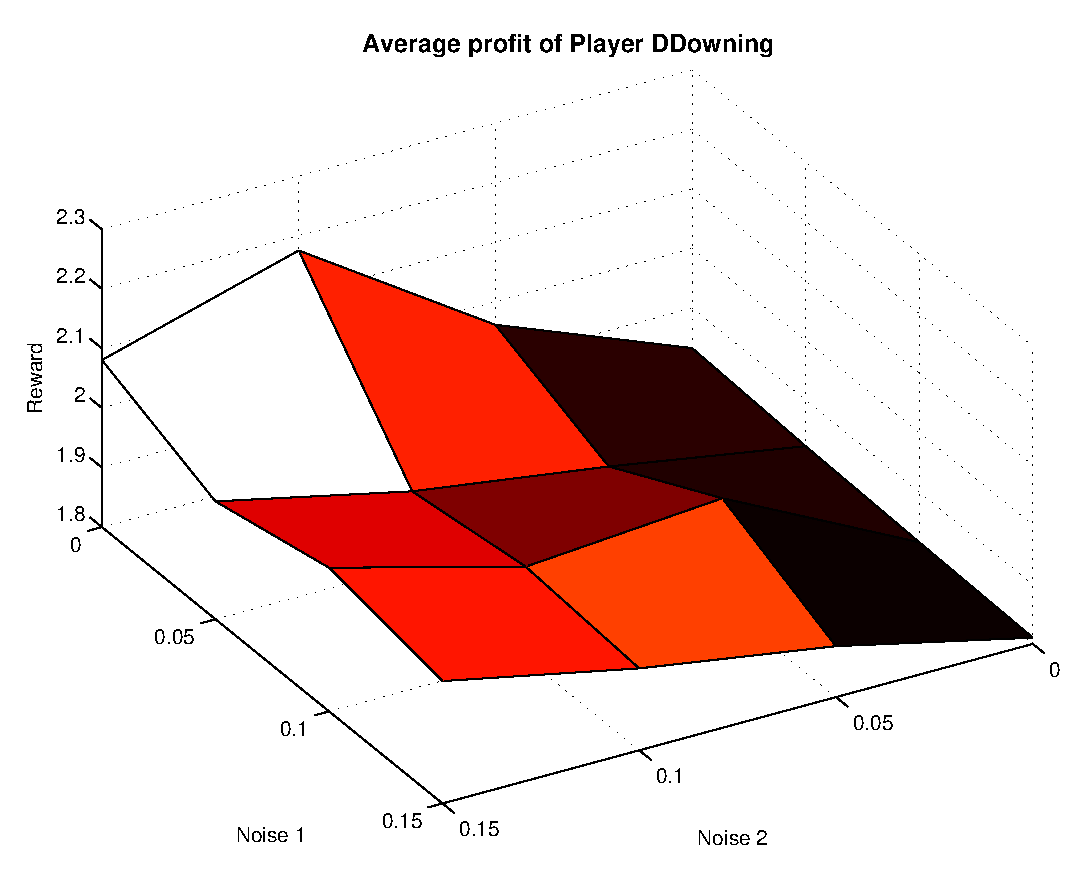
\includegraphics[width=\textwidth]{pics/simulation1/Reward_vs_Noise_of_Player_DDowning}
\end{minipage}
\hfill
\begin{minipage}[hbt]{0.3\textwidth}
	\centering
	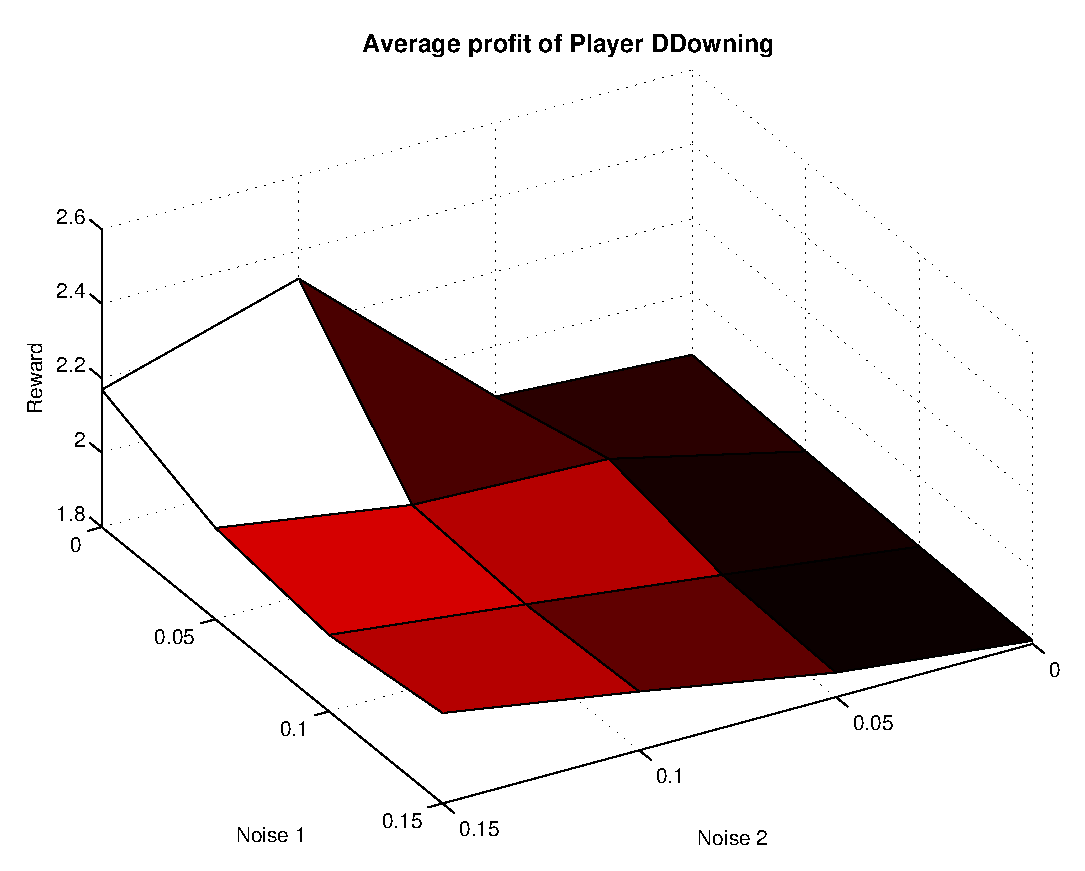
\includegraphics[width=\textwidth]{pics/simulation2/Reward_vs_Noise_of_Player_DDowning}
\end{minipage}

\end{figure}

If noise1 is zero, then \verb0CDO0 performs stronger than \verb0DDO0. \verb0DDO0 performs generally poorly with high noise2 and no noise1 there is a slight performance gain. At no noise \verb0DDO0 outperforms \verb0CDO0 against \verb0COOP0 and \verb0WAT0, but is much worse against all \verb0TFT0 mutants and \verb0FRI0. noise2 improves the performance of \verb0DDO0 against the \verb0TFT0 mutants a little. In the individual parings it seems that \verb0DDO0 can end up in either mutual rejection or mutual cooperation. The decision where they end up seems to be random. For example at noise2=0.15 mutual cooperation appears in \verb0TFT0 and \verb0TF2T0, but not in \verb0DIE0 and \verb0JOSS0, while at noise2=0.1 it is the other way around.

\begin{table}[h]
 \begin{center}
\caption{Cooperation of CDO depending on the noise} \vspace{3mm}
\begin{tabular}{|l|c|c|c|c|c|}
\hline
   	& noise2 = 0 & noise2 = 0.05& noise2 = 0.1& noise2 = 0.15 \\
  \hline
  noise1 = 0 	&      0.7507  &  0.6013 &   0.7660 &  0.6504 \\
 \hline
  noise1 = 0.05	 &           0.1210  &  0.1711  &  0.0829 &  0.0507 \\
 \hline
  noise1 = 0.10 	&          0.1169   & 0.0507 &   0.0508  &  0.0508 \\
 \hline
  noise1 = 0.15 	&        0.0507  &  0.0745 &   0.0504 &  0.0505 \\
 \hline
\end{tabular}
 \end{center}
\end{table}

\begin{table}[h]
 \begin{center}
\caption{Cooperation of DDO depending on the noise} \vspace{3mm}
\begin{tabular}{|l|c|c|c|c|c|}
\hline
   	& noise2 = 0 & noise2 = 0.05& noise2 = 0.1& noise2 = 0.15 \\
  \hline
  noise1 = 0 	&        0.0500  &  0.1499&   0.2997  &  0.3500 \\
 \hline
  noise1 = 0.05	 &              0.0500   & 0.0501  &  0.0517  & 0.0502 \\
 \hline
  noise1 = 0.10 	&             0.0500 &   0.1110  &  0.0503  &  0.0502 \\
 \hline
  noise1 = 0.15 	&          0.0501  &  0.0501 &   0.0501  &  0.0502 \\
 \hline
\end{tabular}
 \end{center}
\end{table}

\verb0DDO0 seems to reject almost all the time, while \verb0CDO0 rejects most of the time if noise1 is greater than 0. A problem of Downing is that it compares decisions that happen at the same time, but at this time the opponent does not know Downing's decision, so his decision can only be dependent on Downing's past decisions.


\subsubsection{Tit for Tat with Reputation}
The player's performance is shown in figure~\ref{pic player tftwr}.\\
\begin{figure}[h]
	\caption{Reward plot of TFTR}
	\label{pic player tftwr}
\begin{minipage}[hbt]{0.65\textwidth}
	\centering
	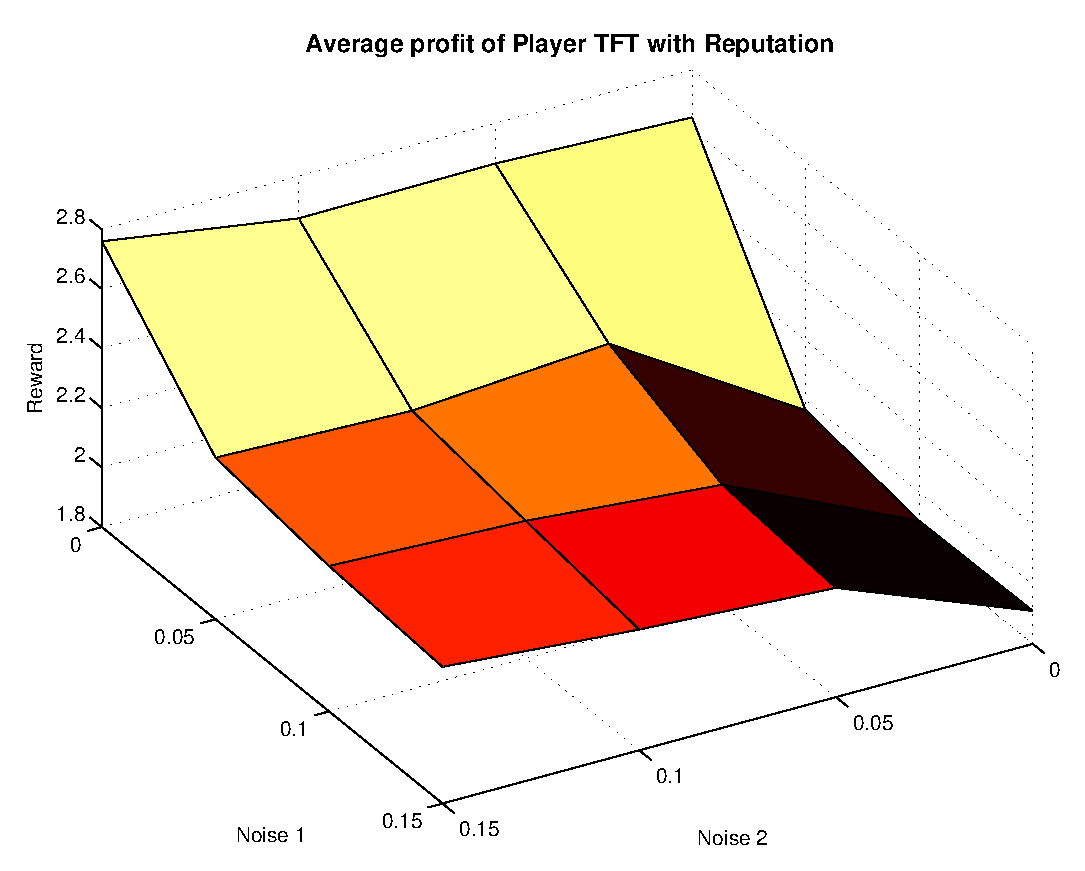
\includegraphics[width=\textwidth]{pics/simulation1/Reward_vs_Noise_of_Player_TFT_with_Reputation}
\end{minipage}
\hfill
\begin{minipage}[hbt]{0.3\textwidth}
	\centering
	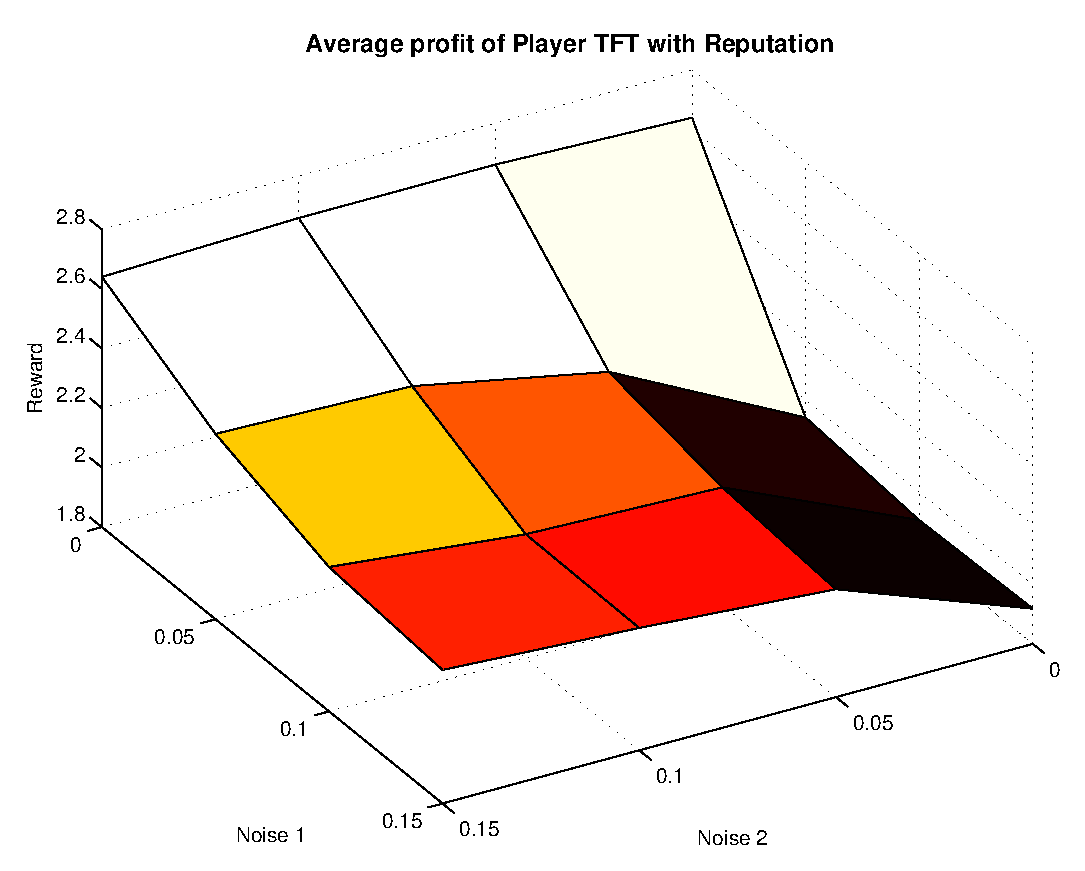
\includegraphics[width=\textwidth]{pics/simulation2/Reward_vs_Noise_of_Player_TFT_with_Reputation}
\end{minipage}

\end{figure}

There were too many unfriendly players, that any player could have been friendly enough so that this player would have looked over a defection. The only player that would cooperate enough is \verb0COOP0. Against this player the number of cooperations were higher than the one of \verb0TFT0, but because \verb0COOP0 is an exploitable player, this actually hurt this strategy.
In an environment where most players are cooperating this player could theoretically be exploited.

\begin{table}[h]
 \begin{center}
\caption{Cooperation of TFTR depending on the noise} \label{tab:tftr}\vspace{3mm}
\begin{tabular}{|l|c|c|c|c|c|}
\hline
   	& noise2 = 0 & noise2 = 0.05& noise2 = 0.1& noise2 = 0.15 \\
  \hline
  noise1 = 0 	&           0.8059  & 0.8218&    0.8375   & 0.8440 \\
 \hline
  noise1 = 0.05	 &     0.8059  &  0.8218 &   0.8375   & 0.84402 \\
 \hline
  noise1 = 0.10 	&     0.3476  &  0.4939  &  0.5341  &  0.5942 \\
 \hline
  noise1 = 0.15 	&    0.3202 &   0.4402 &   0.4906 &   0.5349 \\
 \hline
\end{tabular}
 \end{center}
\end{table}

The values in table~\ref{tab:tftr} are very similar to the results of \verb0TFT0.\\

\subsubsection{Strategy Switcher}
The player's performance is shown in figure~\ref{pic player ss}.\\
\begin{figure}[h]
	\caption{Reward plot of SSW}
	\label{pic player ss}
\begin{minipage}[hbt]{0.65\textwidth}
	\centering
	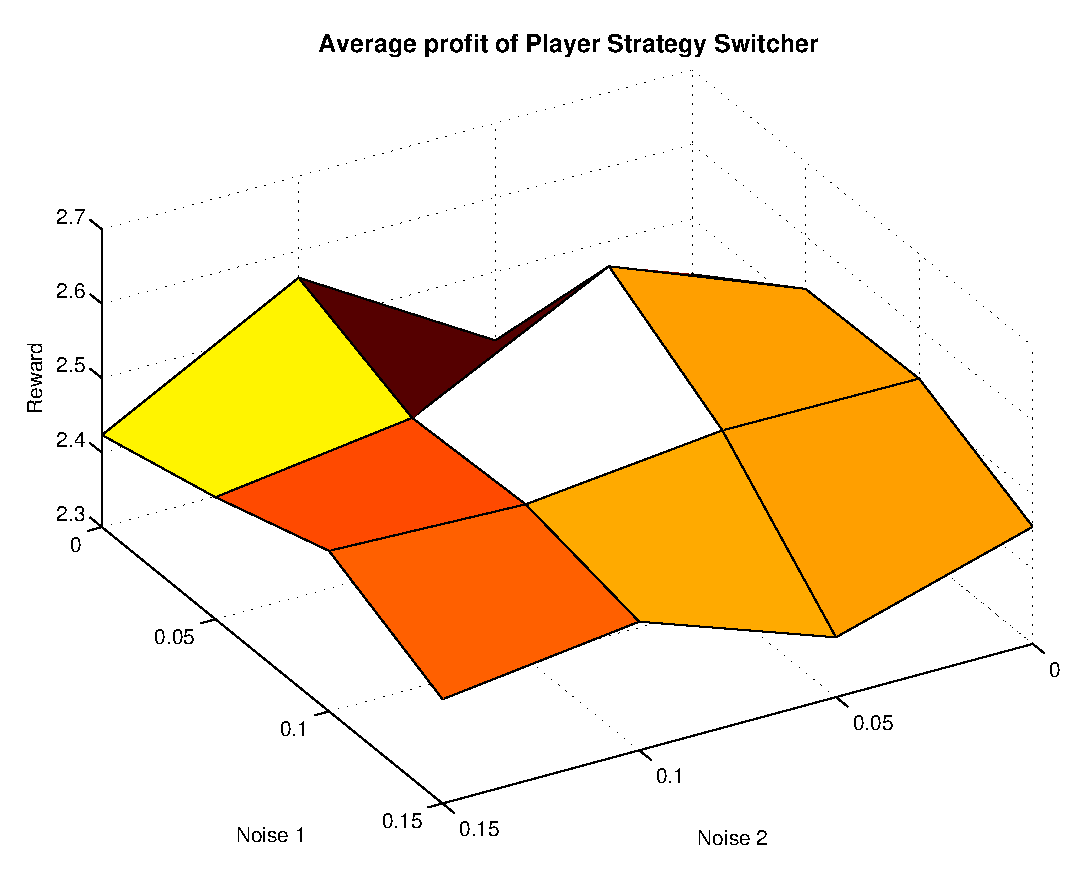
\includegraphics[width=\textwidth]{pics/simulation1/Reward_vs_Noise_of_Player_Strategy_Switcher}
\end{minipage}
\hfill
\begin{minipage}[hbt]{0.3\textwidth}
	\centering
	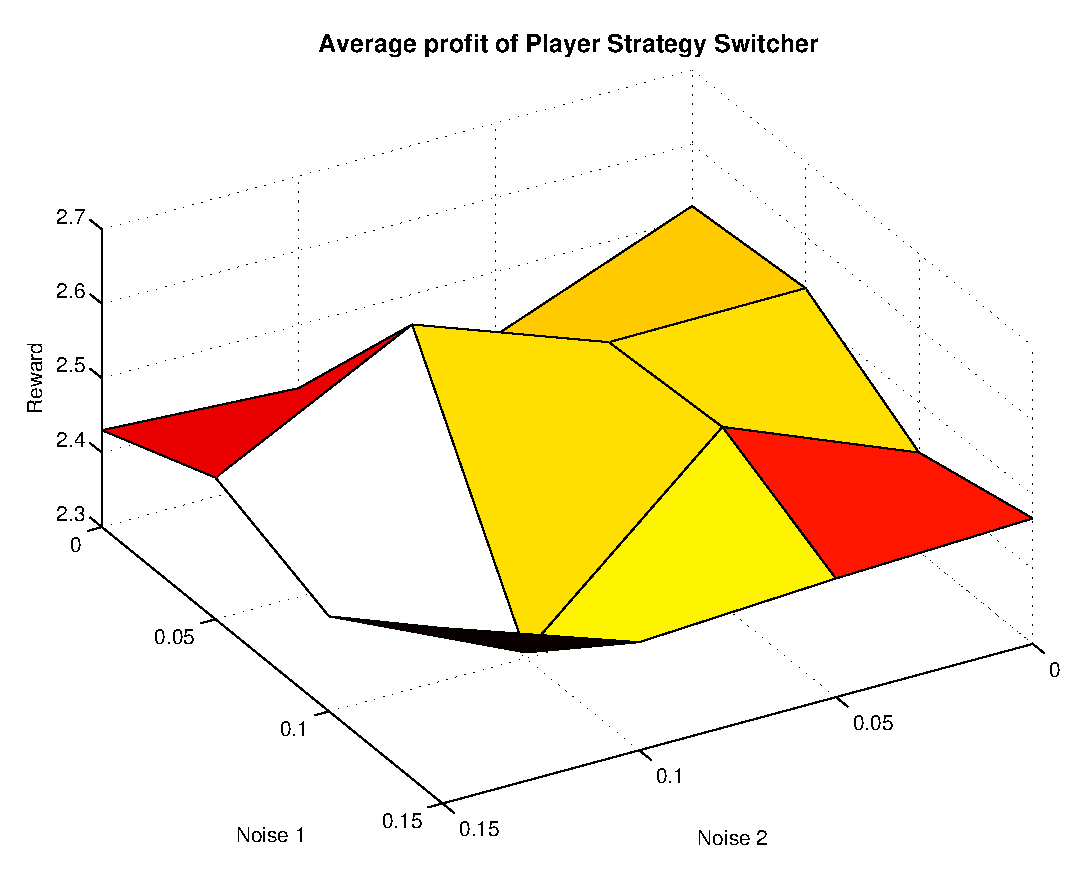
\includegraphics[width=\textwidth]{pics/simulation2/Reward_vs_Noise_of_Player_Strategy_Switcher}
\end{minipage}

\end{figure}

This player was by far the strongest player before the Downing players were added to the simulation. In the final simulation he is strong in fields, where the noise is large as is performance is not impacted by noise. The disadvantage comes from trying out different strategies in the beginning. In the case of no noise this means that \verb0FRI0 will always defect. In the case of Downing mutants this seems to result in defections from the Downing players. Before these Downing players were added this player outperformed \verb0TFT0 by a huge margin, even at zero noise. The strength of this player comes from his ability to cooperate with \verb0TFT0 mutants and exploit exploitable players. This player might even be stronger if better strategies were given to his arsenal. Currently he has \verb0COOP0, \verb0DEF0, \verb0TFT0, \verb0TF2T0 and \verb0PAV0 as his choices. A more efficient choice might have been \verb0LTFT0 and \verb0DEF0. Currently it also contains exploitable strategies (\verb0TF2T0), so the player could be exploited.\\

In long simulations the player can benefit from having the optimal strategy, while in short simulations he spends a large amount of the time trying out strategies that might not be very strong.

\begin{table}[h]
 \begin{center}
\caption{Cooperation of SSW depending on the noise} \vspace{3mm}
\begin{tabular}{|l|c|c|c|c|c|}
\hline
   	& noise2 = 0 & noise2 = 0.05& noise2 = 0.1& noise2 = 0.15 \\
  \hline
  noise1 = 0 	&     0.5164 &   0.5430  &  0.4803  &  0.4659 \\
 \hline
  noise1 = 0.05	 &    0.5164  &  0.5430   & 0.4803   & 0.4659 \\
 \hline
  noise1 = 0.10 	&    0.5098  &  0.5520  &  0.4497 &   0.4888 \\
 \hline
  noise1 = 0.15 	&        0.5097  &  0.5318 &   0.4675 &   0.4467 \\
 \hline
\end{tabular}
 \end{center}
\end{table}

The number of cooperations is rather low, but also does not change very much with the noise. This is most likely, because this player actively looks if an opponent is exploitable.\\

Traits of the player:


\renewcommand{\labelitemi}{}
\begin{itemize}
	\item + Can exploit others
	\item + noise doesn't impact performance
	\item + Very adaptive
	\item + Strong in long simulations
	\item - Exploitable himself
	\item - Exploring defective moves can backfire (\verb0FRI0)
	\item - Is hard to read initially, this might trigger defections
	\item - Weak in short simulations
\end{itemize}
\renewcommand{\labelitemi}{$\bullet$}

\subsubsection{Lookback CDowning and Lookback DDowning}
The two players' performance is shown in figure~\ref{pic player lbcd} (\verb0LCDO0) and figure~\ref{pic player lbdd} (\verb0LDDO0).\\
\begin{figure}[h]
	\caption{Reward plot of LCDO}
	\label{pic player lbcd}
\begin{minipage}[hbt]{0.65\textwidth}
	\centering
	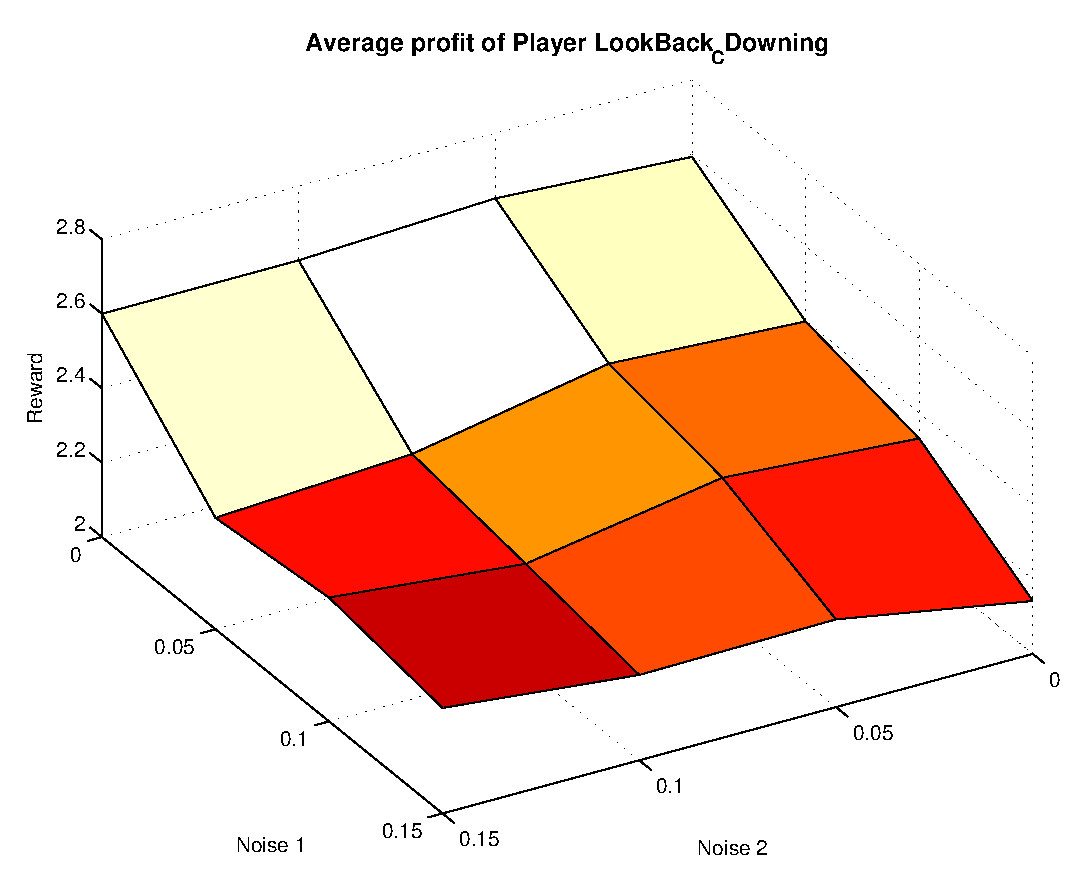
\includegraphics[width=\textwidth]{pics/simulation1/Reward_vs_Noise_of_Player_LookBack_CDowning}
\end{minipage}
\hfill
\begin{minipage}[hbt]{0.3\textwidth}
	\centering
	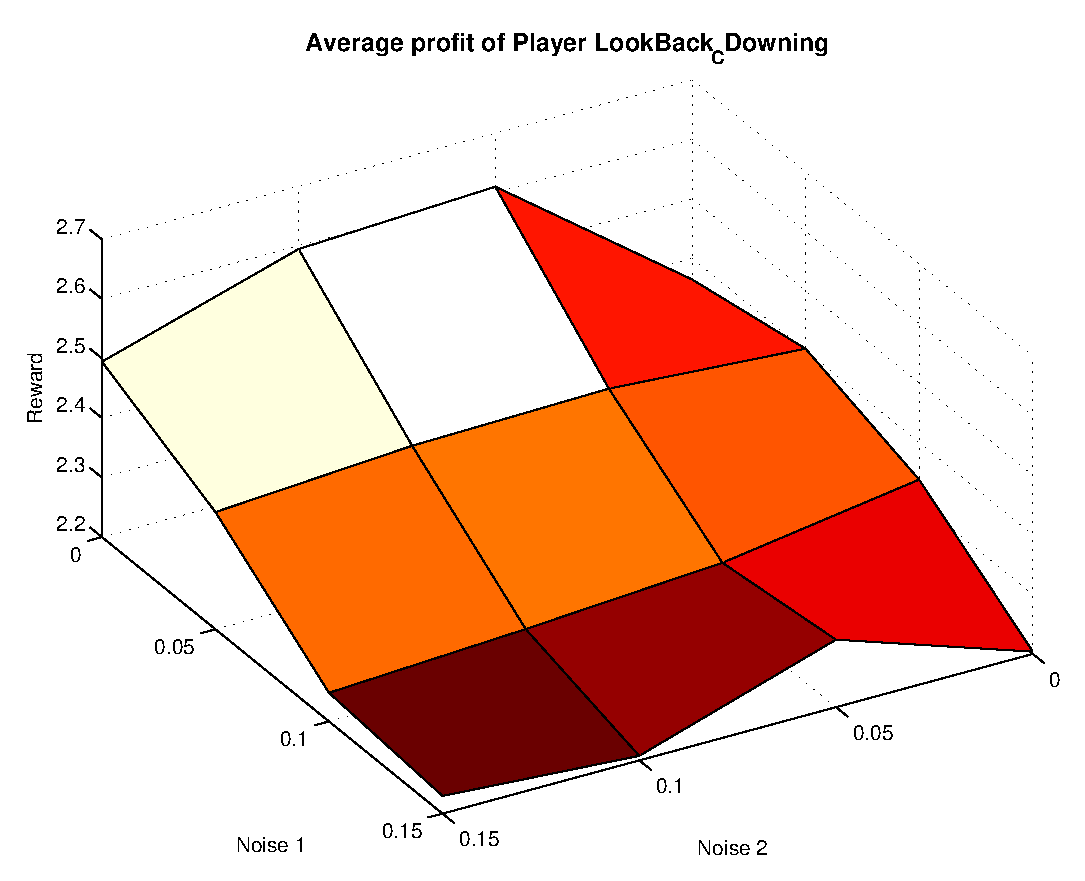
\includegraphics[width=\textwidth]{pics/simulation2/Reward_vs_Noise_of_Player_LookBack_CDowning}
\end{minipage}

\end{figure}

\begin{figure}[h]
	\caption{Reward plot of LDDO}
	\label{pic player lbdd}
\begin{minipage}[hbt]{0.65\textwidth}
	\centering
	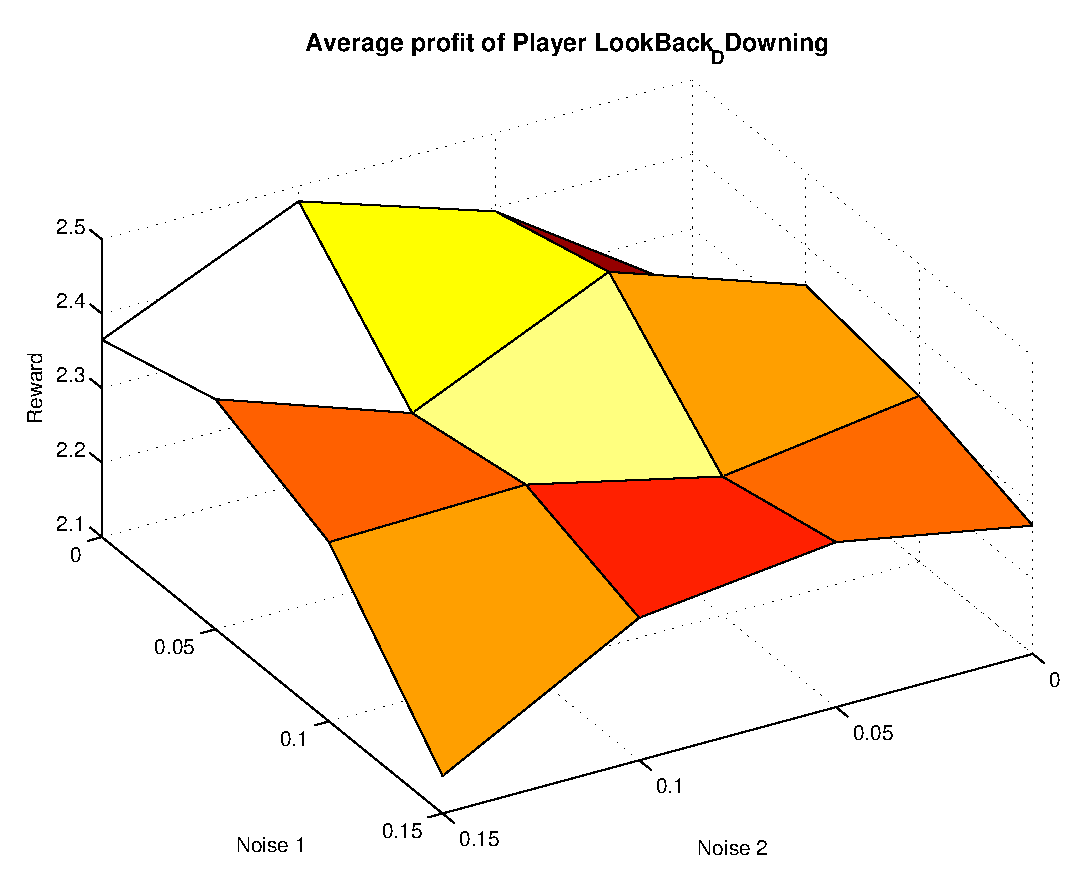
\includegraphics[width=\textwidth]{pics/simulation1/Reward_vs_Noise_of_Player_LookBack_DDowning}
\end{minipage}
\hfill
\begin{minipage}[hbt]{0.3\textwidth}
	\centering
	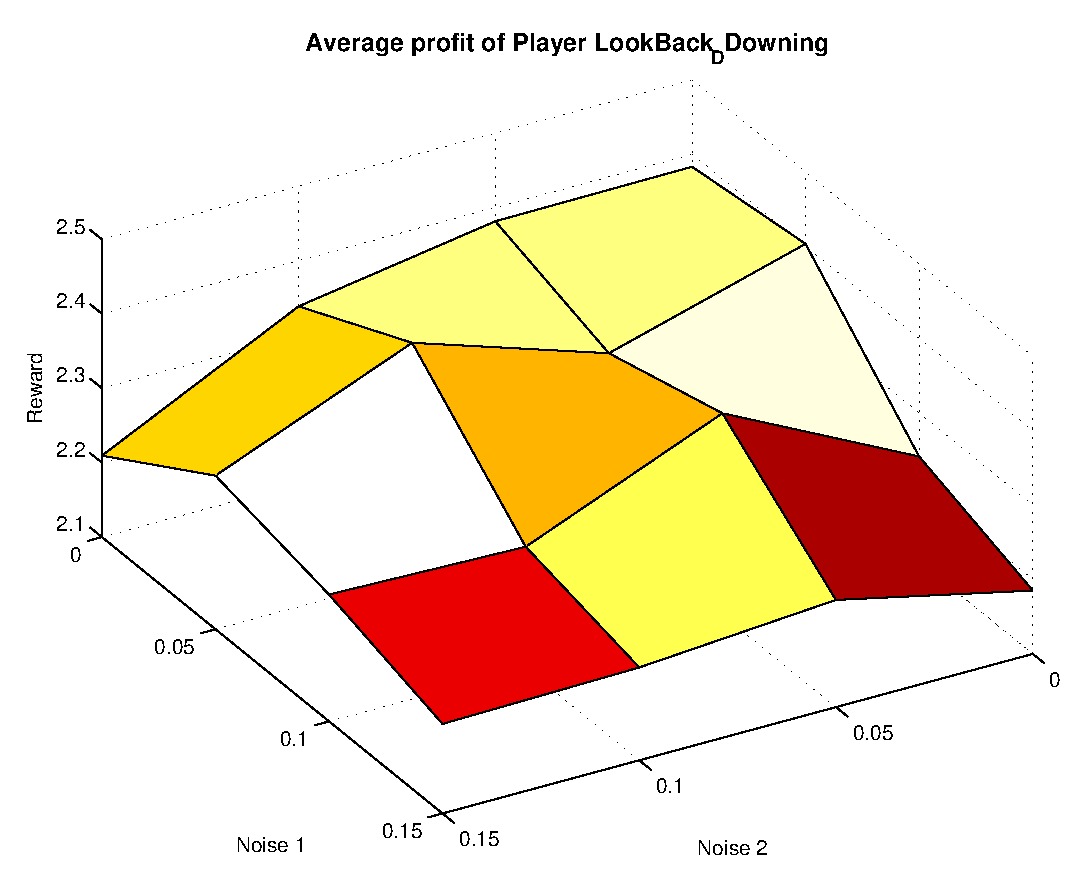
\includegraphics[width=\textwidth]{pics/simulation2/Reward_vs_Noise_of_Player_LookBack_DDowning}
\end{minipage}

\end{figure}

Generally both looking back Downings are stronger than the none looking back ones. If noise1 is zero, \verb0LCDO00 mutant has again a higher performance. Comparing the second last move with the last move of the opponent seems to be the better way to correlate your actions with your opponent's actions. \verb0LDDO0 seems to be very resilient to noise.

At zero noise \verb0LCDO0 performs well with most players, except \verb0EVO0, \verb0SS0, and some Downing mutants. With noise the performance against \verb0FRI0 and some Downing mutants that went well before drops. The overall performance however stays higher than \verb0TFT0.

\begin{table}[h]
 \begin{center}
\caption{Cooperation of LCDO depending on the noise} \vspace{3mm}
\begin{tabular}{|l|c|c|c|c|c|}
\hline
   	& noise2 = 0 & noise2 = 0.05& noise2 = 0.1& noise2 = 0.15 \\
  \hline
  noise1 = 0 	&     0.7507   & 0.6511 &   0.6509&    0.7010 \\
 \hline
  noise1 = 0.05	 &      0.4385 &   0.4405 &   0.4376 &   0.4329 \\
 \hline
  noise1 = 0.10 	&      0.4297  &  0.3865  &  0.3787  &  0.3696 \\
 \hline
  noise1 = 0.15 	&    0.3814  &  0.4120 &   0.3682  &  0.3271 \\
 \hline
\end{tabular}
 \end{center}
\end{table}

\begin{table}[h]
 \begin{center}
\caption{Cooperation of LDDO depending on the noise} \vspace{3mm}
\begin{tabular}{|l|c|c|c|c|c|}
\hline
   	& noise2 = 0 & noise2 = 0.05& noise2 = 0.1& noise2 = 0.15 \\
  \hline
  noise1 = 0 	&   0.4037 &   0.4563 &   0.4071   & 0.4762 \\
 \hline
  noise1 = 0.05	 &     0.4386  &  0.3912 &   0.4303   & 0.3848 \\
 \hline
  noise1 = 0.10 	&      0.3864   & 0.4025  &  0.3784 &  0.3827 \\
 \hline
  noise1 = 0.15 	&    0.3868 &   0.3262 &   0.3840  &  0.3769 \\
 \hline
\end{tabular}
 \end{center}
\end{table}

The number of cooperations is in general much higher, than for variants, whihk do not look back. For noise1 greater than zero about 40\% cooperative moves remain, while \verb0CDO0 and \verb0DDO0 fall down to 5-10\% cooperative moves. The average rewards for these players are also 0.2-0.5 higher then their not looking back counterparts.


\subsubsection{Watcher}
The player's performance is shown in figure~\ref{pic player watcher}.\\
\begin{figure}[h]
	\caption{Reward plot of WAT}
	\label{pic player watcher}
\begin{minipage}[hbt]{0.65\textwidth}
	\centering
	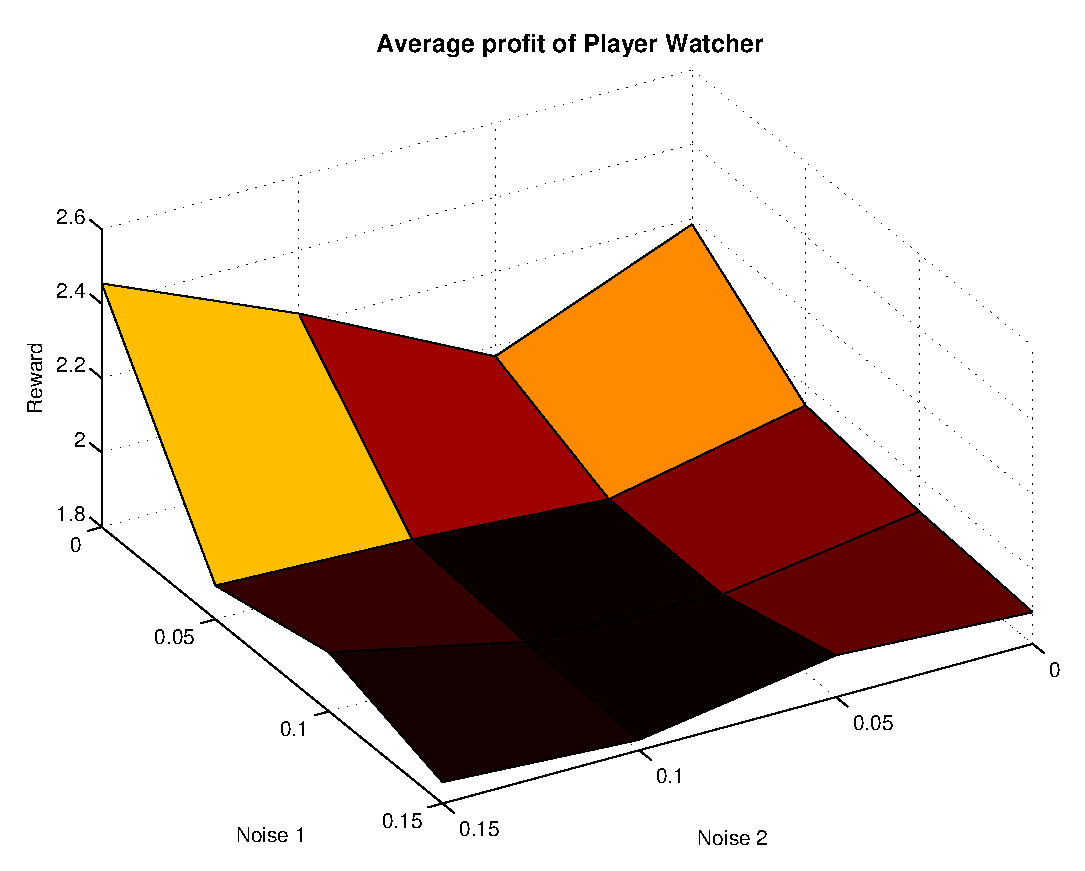
\includegraphics[width=\textwidth]{pics/simulation1/Reward_vs_Noise_of_Player_Watcher}
\end{minipage}
\hfill
\begin{minipage}[hbt]{0.3\textwidth}
	\centering
	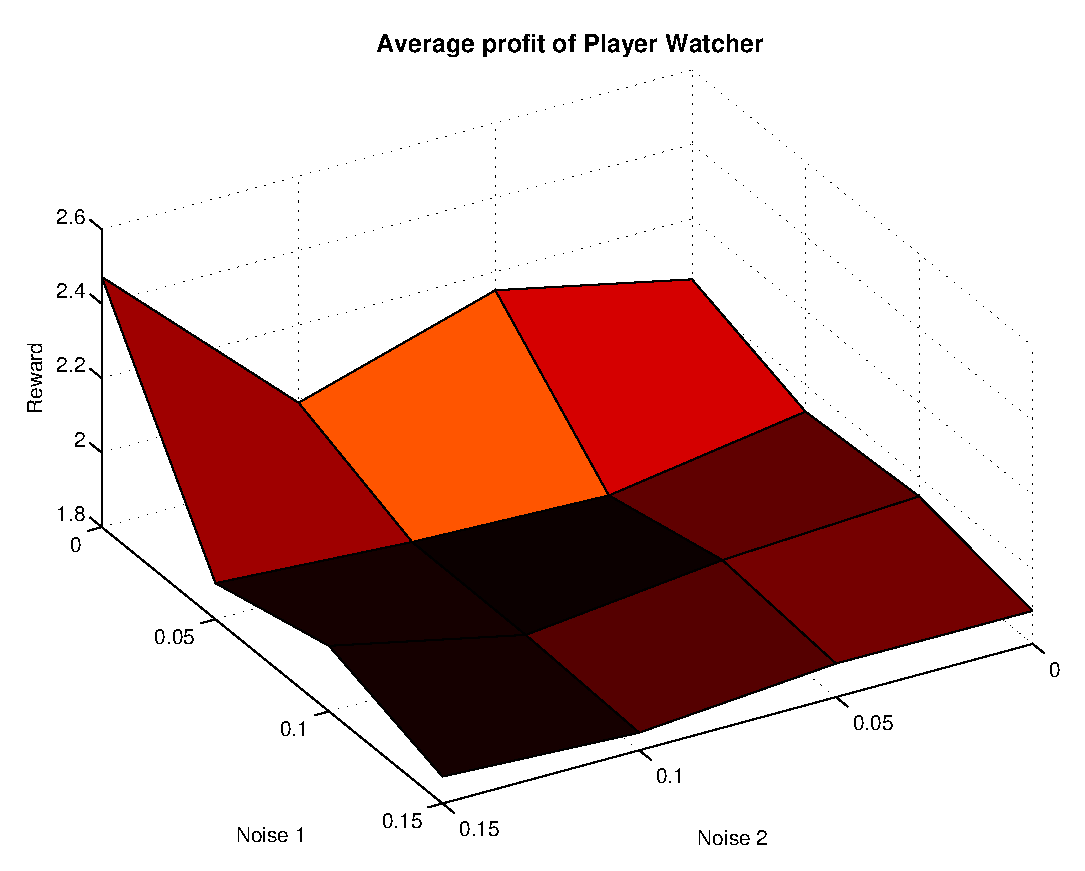
\includegraphics[width=\textwidth]{pics/simulation2/Reward_vs_Noise_of_Player_Watcher}
\end{minipage}

\end{figure}

This player generally does not perform very strong. It does not respond and can therefore be exploited. It also does not take the local situation into account. It will betray \verb0FRI0 even in no noise, because in short term this is successful. After that the player copies strategies that were cooperative the whole time, while \verb0FRI0 is defecting. There is point of higher performance, where noise2 is 0.15 and noise1 is zero. For some reason it performs strong against the looking back Downing algorithms.\\

\begin{table}[h]
 \begin{center}
\caption{Cooperation of WAT depending on the noise} \vspace{3mm}
\begin{tabular}{|l|c|c|c|c|c|}
\hline
   	& noise2 = 0 & noise2 = 0.05& noise2 = 0.1& noise2 = 0.15 \\
  \hline
  noise1 = 0 	&       0.5399  &  0.4704  &  0.4298 &   0.4020 \\
 \hline
  noise1 = 0.05	 &        0.4569  &  0.3854 &   0.3544  & 0.3552 \\
 \hline
  noise1 = 0.10 	&         0.4297 &   0.3691  &  0.3522  &  0.3576 \\
 \hline
  noise1 = 0.15 	&       0.4125 &   0.3510&    0.3428  &  0.3504 \\
 \hline
\end{tabular}
 \end{center}
\end{table}

Generally the number of cooperations is rather low, but there are no drastic jumps.

\subsubsection{Evolutionary}
The player's performance is shown in figure~\ref{pic player evo}.\\
\begin{figure}[h]
	\caption{Reward plot of EVO}
	\label{pic player evo}
\begin{minipage}[hbt]{0.65\textwidth}
	\centering
	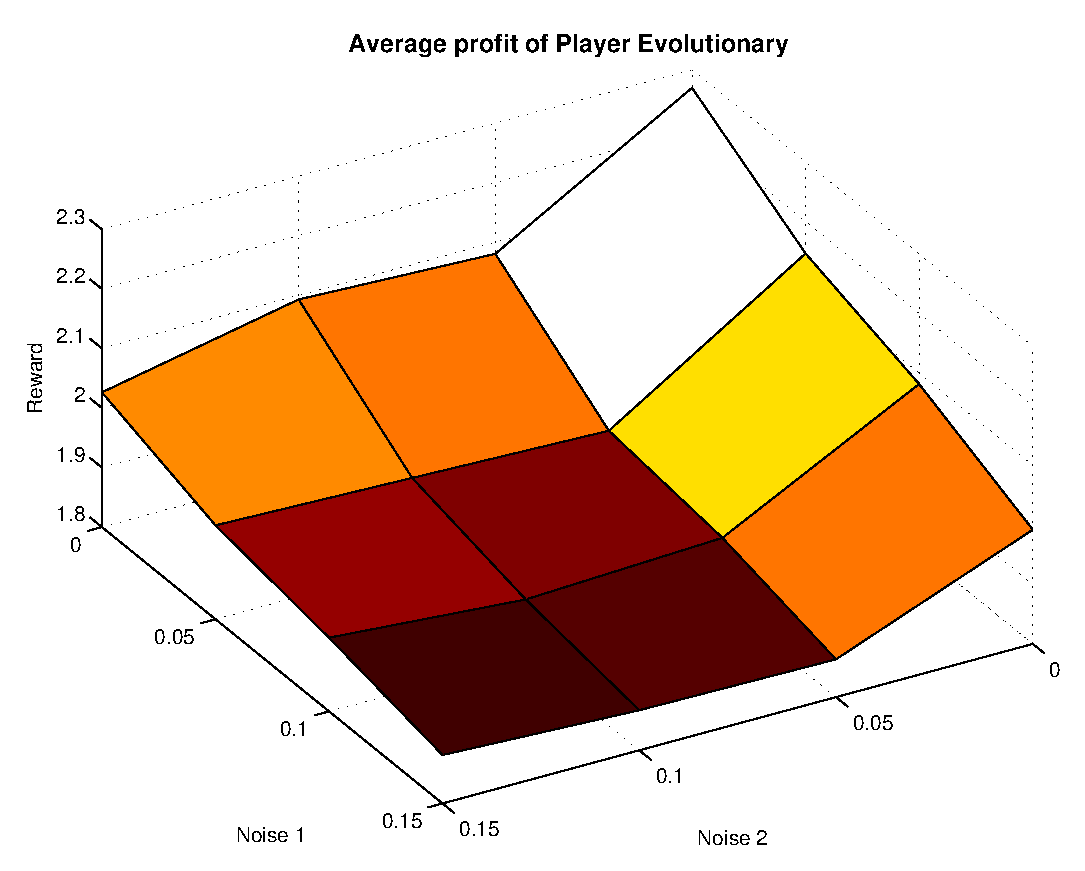
\includegraphics[width=\textwidth]{pics/simulation1/Reward_vs_Noise_of_Player_Evolutionary}
\end{minipage}
\hfill
\begin{minipage}[hbt]{0.3\textwidth}
	\centering
	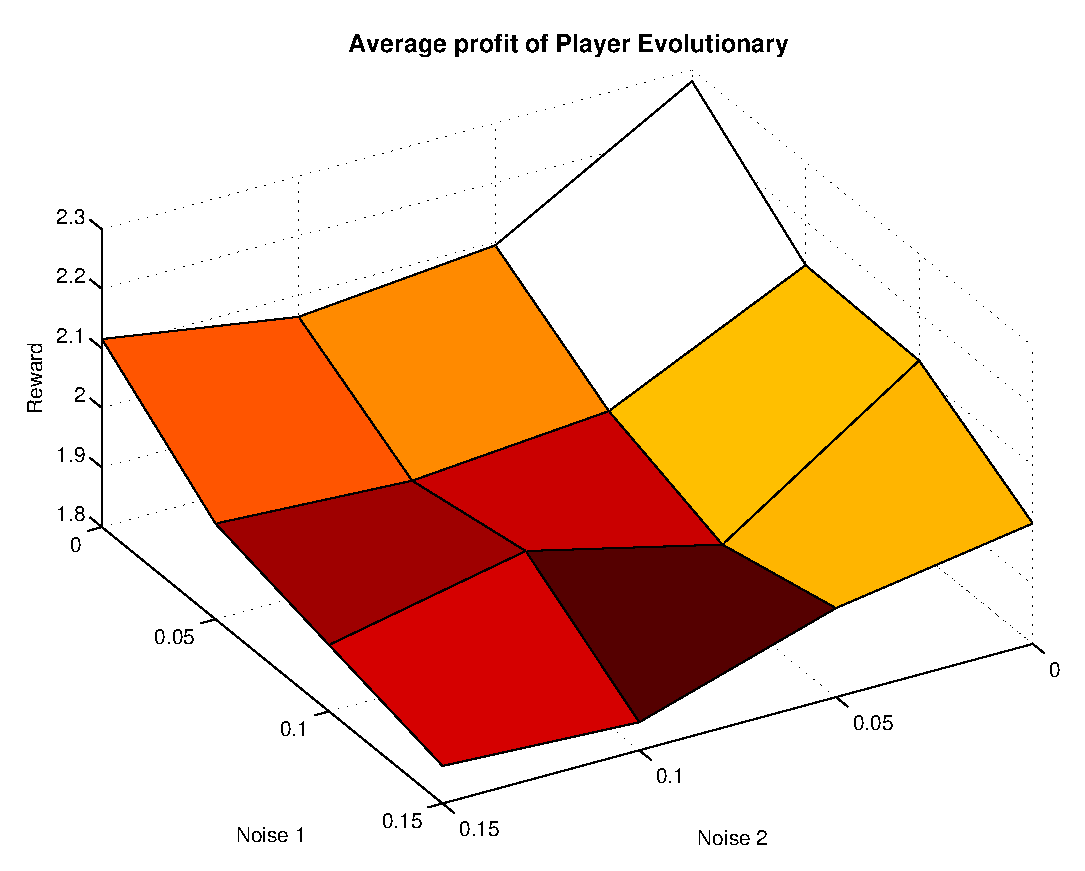
\includegraphics[width=\textwidth]{pics/simulation2/Reward_vs_Noise_of_Player_Evolutionary}
\end{minipage}

\end{figure}

This player performs rather poorly at all noises. Less noise is better for him, because more reliable information allows the player to adjust. Noise generally promotes bad strategies, while they are sorted out when there is little noise. The problem is that this players does add rejections and therefore triggers others rejections. The player himself has a very slow reaction time. Changing his strategy by mutations takes hundreds of turns. This is a timescale the opponents cannot see. This player does not look responsive to the opponents. The player himself can only see the opponents reaction if it is within the segment length that the player tries to optimize. The interesting thing is that this player is able to exploit \verb0TF2T0, he will add defections with mostly one sometimes two cooperative steps between them. It has a performance of 3.65 against \verb0TF2T0 at zero noise.\\

\begin{table}[h]
 \begin{center}
\caption{Cooperation of EVO depending on the noise} \vspace{3mm}
\begin{tabular}{|l|c|c|c|c|c|}
\hline
   	& noise2 = 0 & noise2 = 0.05& noise2 = 0.1& noise2 = 0.15 \\
  \hline
  noise1 = 0 	&         0.4330 & 0.4941  &  0.5151  &  0.4878 \\
 \hline
  noise1 = 0.05	 &          0.3859   & 0.4745 &   0.4860 &   0.4855\\
 \hline
  noise1 = 0.10 	&    0.3987 &   0.4750&    0.4919&    0.4914 \\
 \hline
  noise1 = 0.15 	&     0.3755 &   0.4793  &  0.4733  &  0.4896 \\
 \hline
\end{tabular}
 \end{center}
\end{table}

The decisions seem to be mostly an even mix of defections and cooperations, with a slight preference of defections.\\


\subsubsection{Limited Reconciliation Tit for tat}
The player's performance is shown in figure~\ref{pic player lrtft}.\\
\begin{figure}[h]
	\caption{Reward plot of LTFT}
	\label{pic player lrtft}
\begin{minipage}[hbt]{0.65\textwidth}
	\centering
	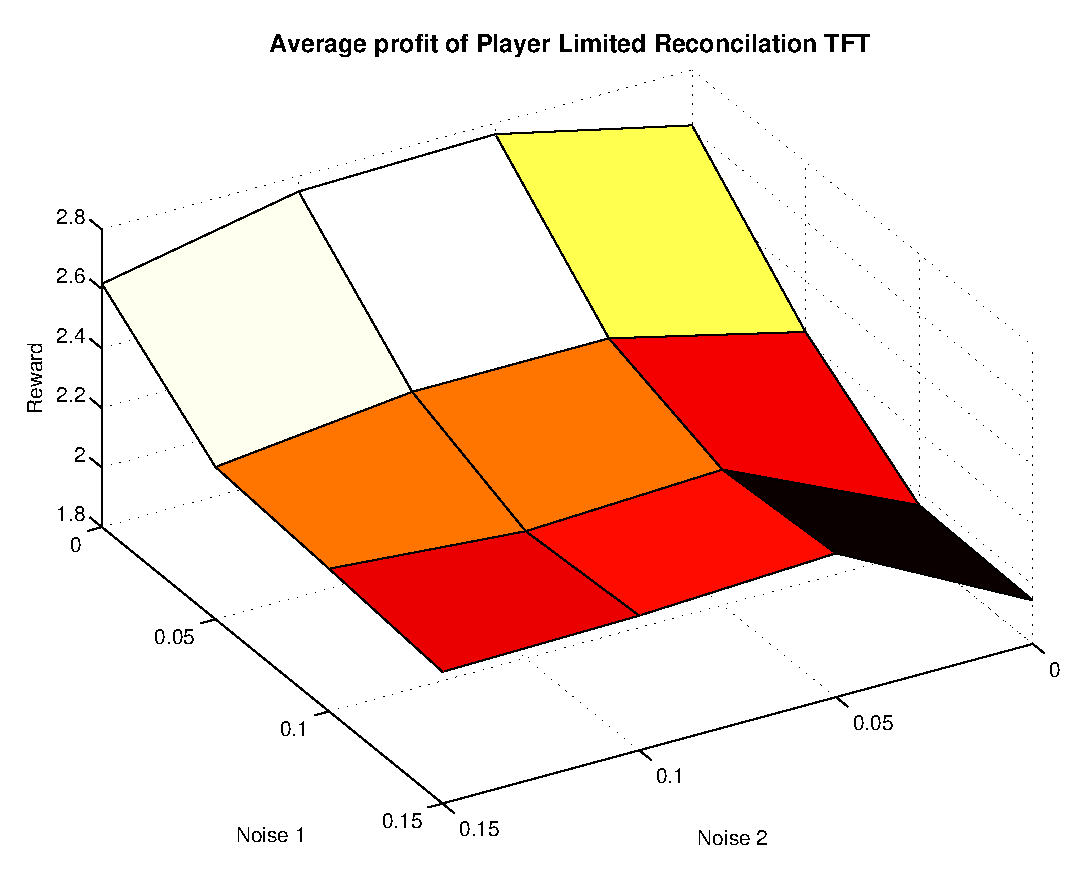
\includegraphics[width=\textwidth]{pics/simulation1/Reward_vs_Noise_of_Player_Limited_Reconcilation_TFT}
\end{minipage}
\hfill
\begin{minipage}[hbt]{0.3\textwidth}
	\centering
	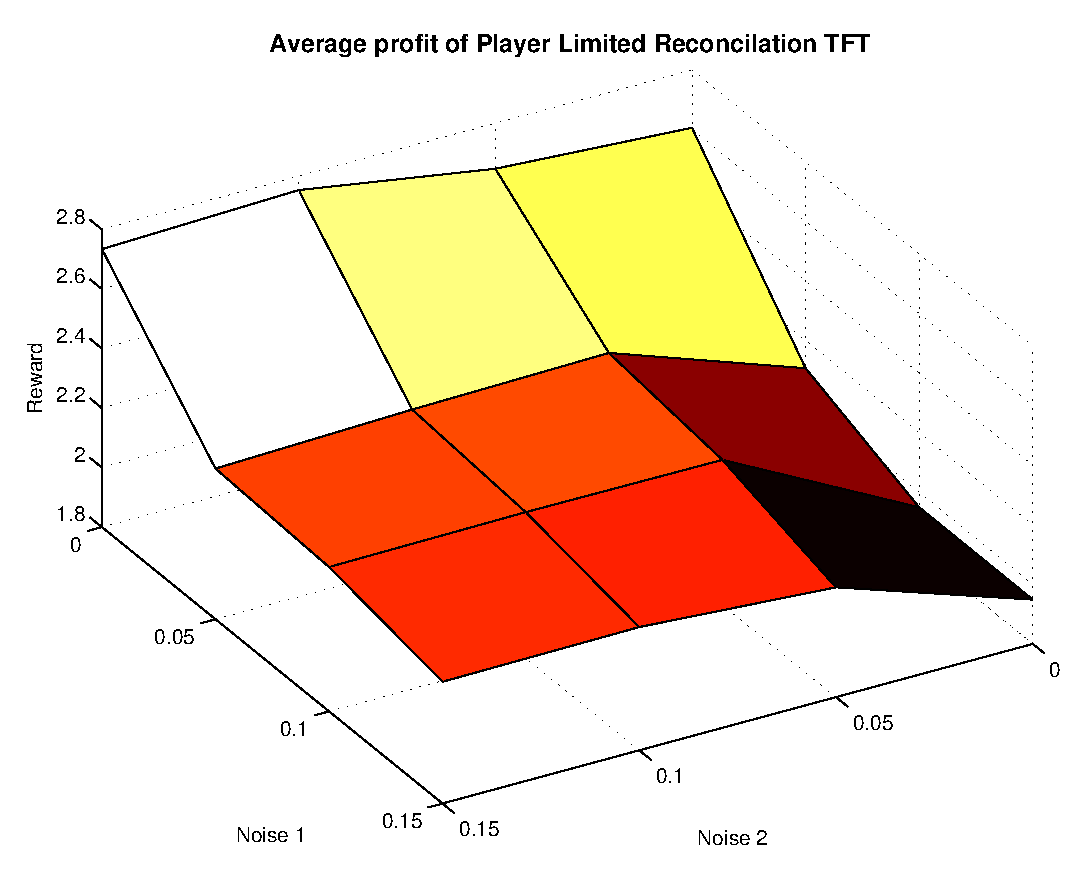
\includegraphics[width=\textwidth]{pics/simulation2/Reward_vs_Noise_of_Player_Limited_Reconcilation_TFT}
\end{minipage}

\end{figure}

At noise1 equal to zero the performance is similar to \verb0TFT0. It does not perform as well as Reconciliation \verb0TFT0 against \verb0JOSS0, therefore it might be wiser to make the time between the reconciliation attempts larger every time, instead of limiting it to 3. Compared to \verb0TFT0 its performance does not break down that much with noise1, this is a property it shares with \verb0DIE0, \verb0TFAT0 and \verb0RTFT0. The fact that the number of reconciliation attempts is limited makes the player stronger against defecting players like \verb0FRI0 (under noise1) and \verb0DEF0.\\

\begin{table}[h]
 \begin{center}
\caption{Cooperation of LTFT depending on the noise} \vspace{3mm}
\begin{tabular}{|l|c|c|c|c|c|}
\hline
   	& noise2 = 0 & noise2 = 0.05& noise2 = 0.1& noise2 = 0.15 \\
  \hline
  noise1 = 0 	&     0.8064&    0.8386 &   0.8942    &0.8976 \\
 \hline
  noise1 = 0.05	 &    0.5084  &  0.6577&    0.6834  &  0.7043\\
 \hline
  noise1 = 0.10 	&0.4254  &  0.6300 &   0.6568 &   0.6822 \\
 \hline
  noise1 = 0.15 	&    0.4208   & 0.5956  &  0.6383  &  0.6648 \\
 \hline
\end{tabular}
 \end{center}
\end{table}

\verb0LTFT0 is not as cooperative as the friendliest \verb0TFT0 mutants \verb0DIE0 and \verb0RTFT0, but more friendly than standard \verb0TFT0 and \verb0TFAT0.\\

Table~\ref{comp} shows the performance of \verb0LTFT0 minus the performance of \verb0TFT0 averaged over all match ups and both simulations:\\

\begin{table}[h]
 \begin{center}
\caption{Comparison of the two players LTFT and TFT} \label{comp}\vspace{3mm}
\begin{tabular}{|l|c|c|c|c|c|}
\hline
   	& noise2 = 0 & noise2 = 0.05& noise2 = 0.1& noise2 = 0.15 \\
  \hline
  noise1 = 0 	&    -0.0317 &   0.0414 &   0.0375&   -0.0892 \\
 \hline
  noise1 = 0.05	 &    0.2235 &  -0.0006  &  0.0310  & -0.0679\\
 \hline
  noise1 = 0.10 	&     0.0438&    0.0340  &  0.0019  &  0.0066 \\
 \hline
  noise1 = 0.15 	&     0.0514  &  0.0720  &  0.0189 &  -0.0312 \\
 \hline
\end{tabular}
 \end{center}
\end{table}

At higher values for noise1, \verb0LTFT0 outperforms \verb0TFT0, while at high noise2 values the reconciliation attempts are not needed, because the noise itself achieves that.

\subsection{Impact of Noise on the whole System}

Figure~\ref{pic player adf} and figure~\ref{pic player asdf} shows the behavior of the average cooperation and the average reward in the system.\\

\begin{figure}[h]
	\caption{Total average cooperation against noise}
	\label{pic player adf}
\begin{minipage}[hbt]{0.65\textwidth}
	\centering
	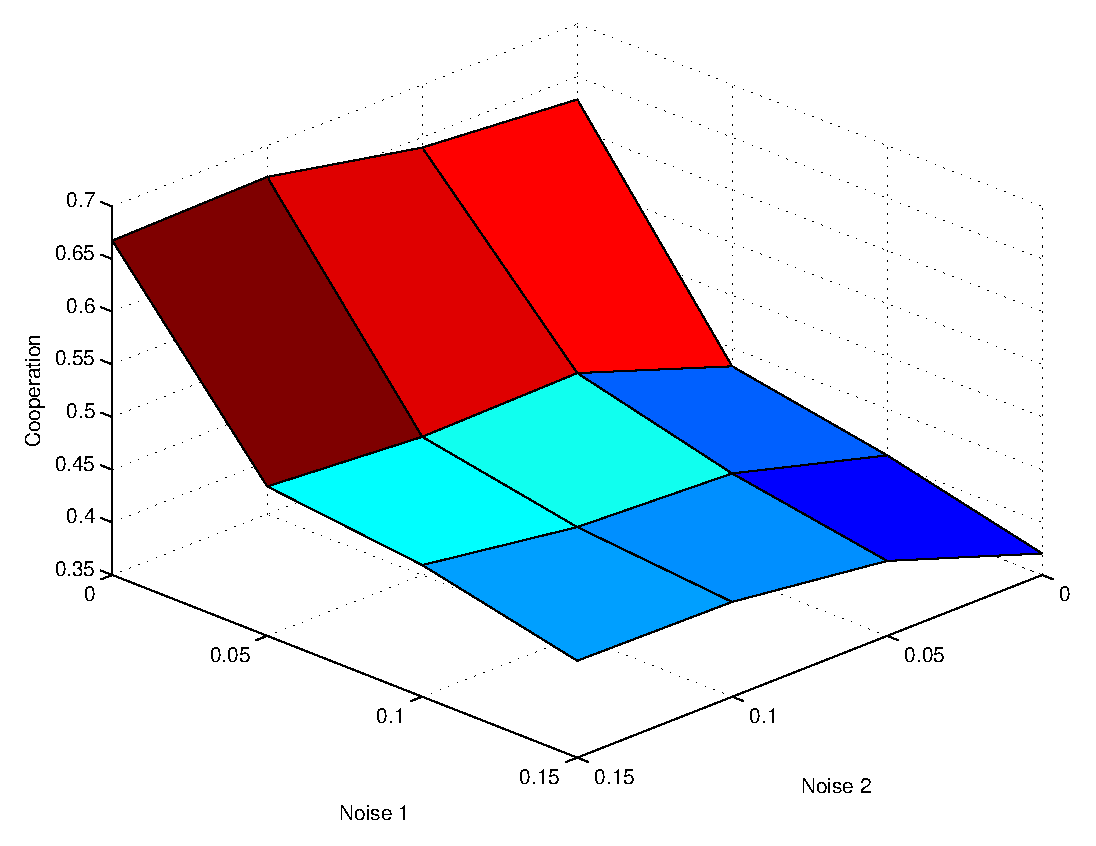
\includegraphics[width=\textwidth]{pics/simulation1/Total_Cooperation_vs_Noise}
\end{minipage}
\hfill
\begin{minipage}[hbt]{0.3\textwidth}
	\centering
	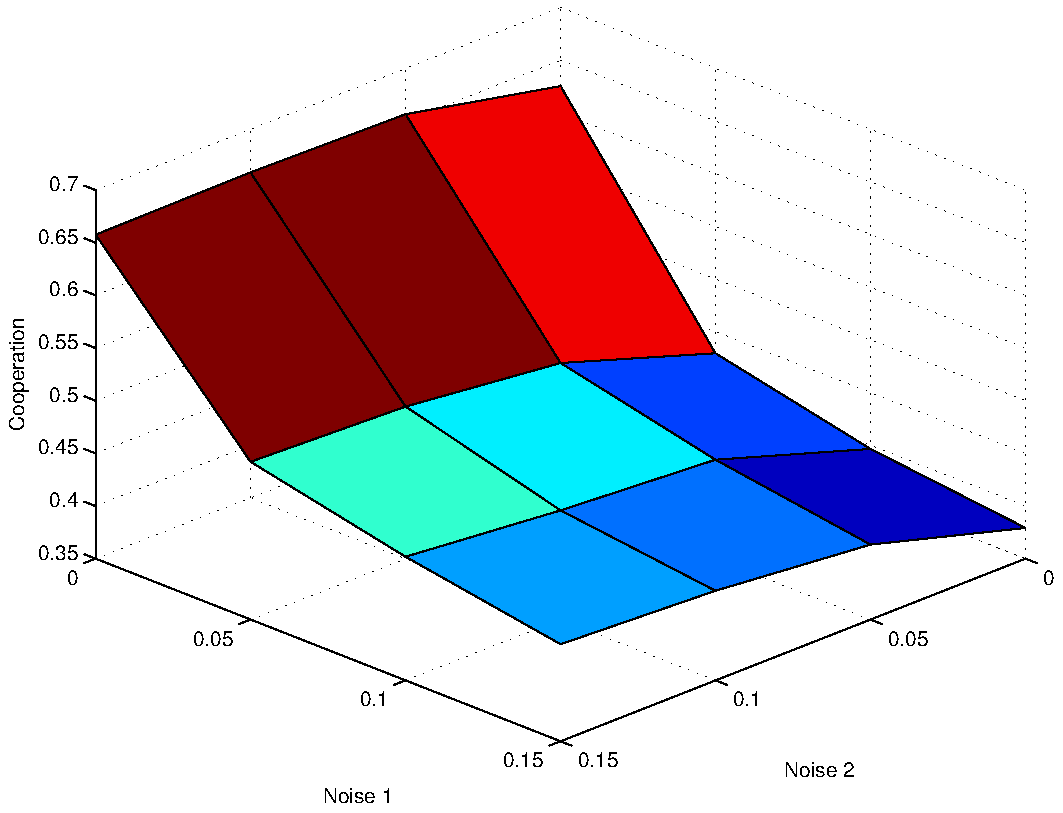
\includegraphics[width=\textwidth]{pics/simulation2/Total_Cooperation_vs_Noise}
\end{minipage}

\end{figure}



\begin{figure}[h]
	\caption{Total average Reward against noise}
	\label{pic player asdf}
\begin{minipage}[hbt]{0.65\textwidth}
	\centering
	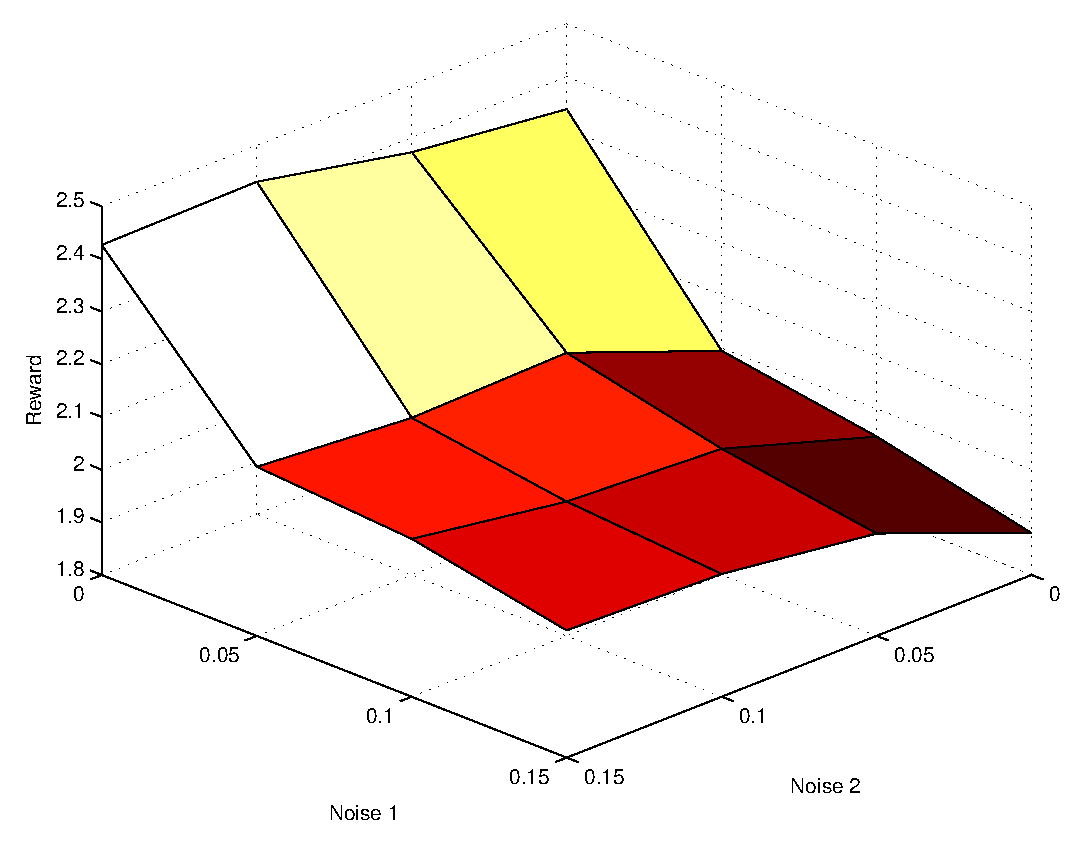
\includegraphics[width=\textwidth]{pics/simulation1/Total_Reward_vs_Noise}
\end{minipage}
\hfill
\begin{minipage}[hbt]{0.3\textwidth}
	\centering
	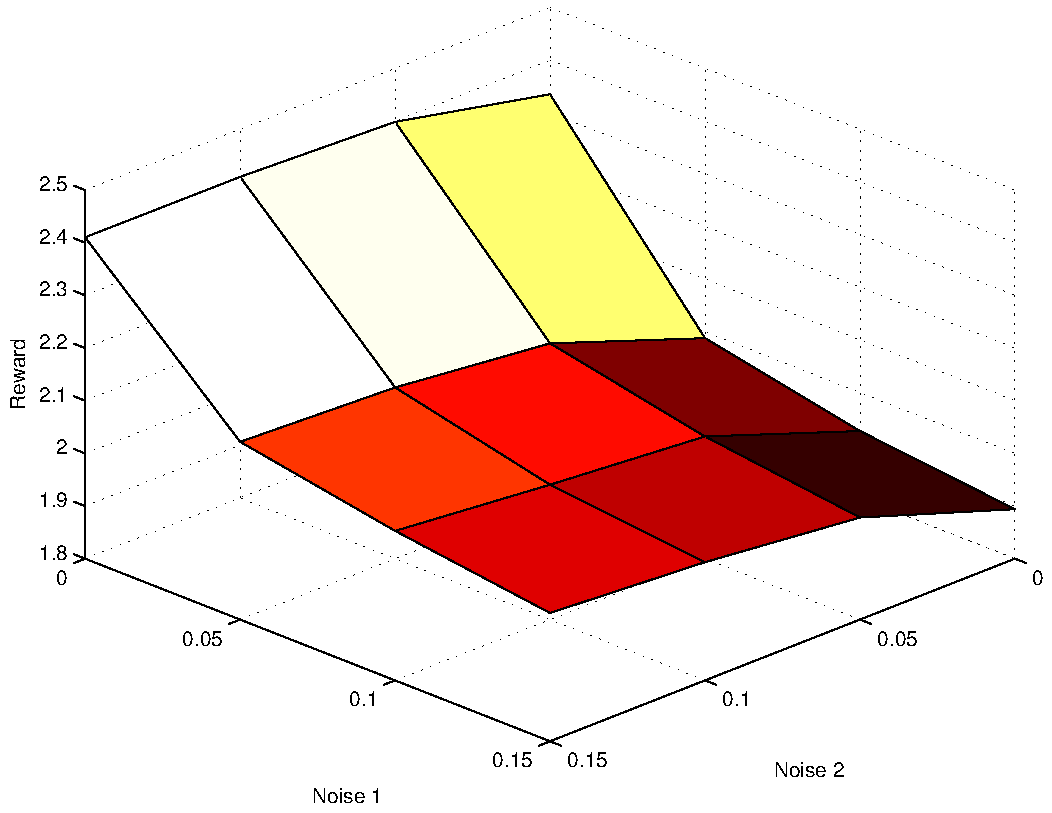
\includegraphics[width=\textwidth]{pics/simulation2/Total_Reward_vs_Noise}
\end{minipage}

\end{figure}


Noise1 seems to destroy cooperation really fast, while noise2 increases it a little. Generally the average reward is the highest if the number of cooperative moves is the highest. The average reward's dependence on the noise looks very similar to the values a typical \verb0TFT0 mutant has. This may be related to the fact, that there were 8 \verb0TFT0 mutants in the simulation. By mean of this, the entire system is acting like a big \verb0TFT0 player.


\subsection{Comparison of the Players}

In figure~\ref{pic player best} the average reward is plotted against the different noise levels (\ref{fig:simul1namedplayer} for simulation 1 and \ref{fig:simul2namedplayer} for simulation 2). The brighter the color, the higher is the average reward. In each cell the player with the highest score is named.\\

\begin{figure}[h]
\caption{Reward versus noise with the best players}
	\label{pic player best}
\begin{minipage}[hbt]{1\textwidth}
	\centering
	\subfloat[Simulation 1]{\label{fig:simul1namedplayer}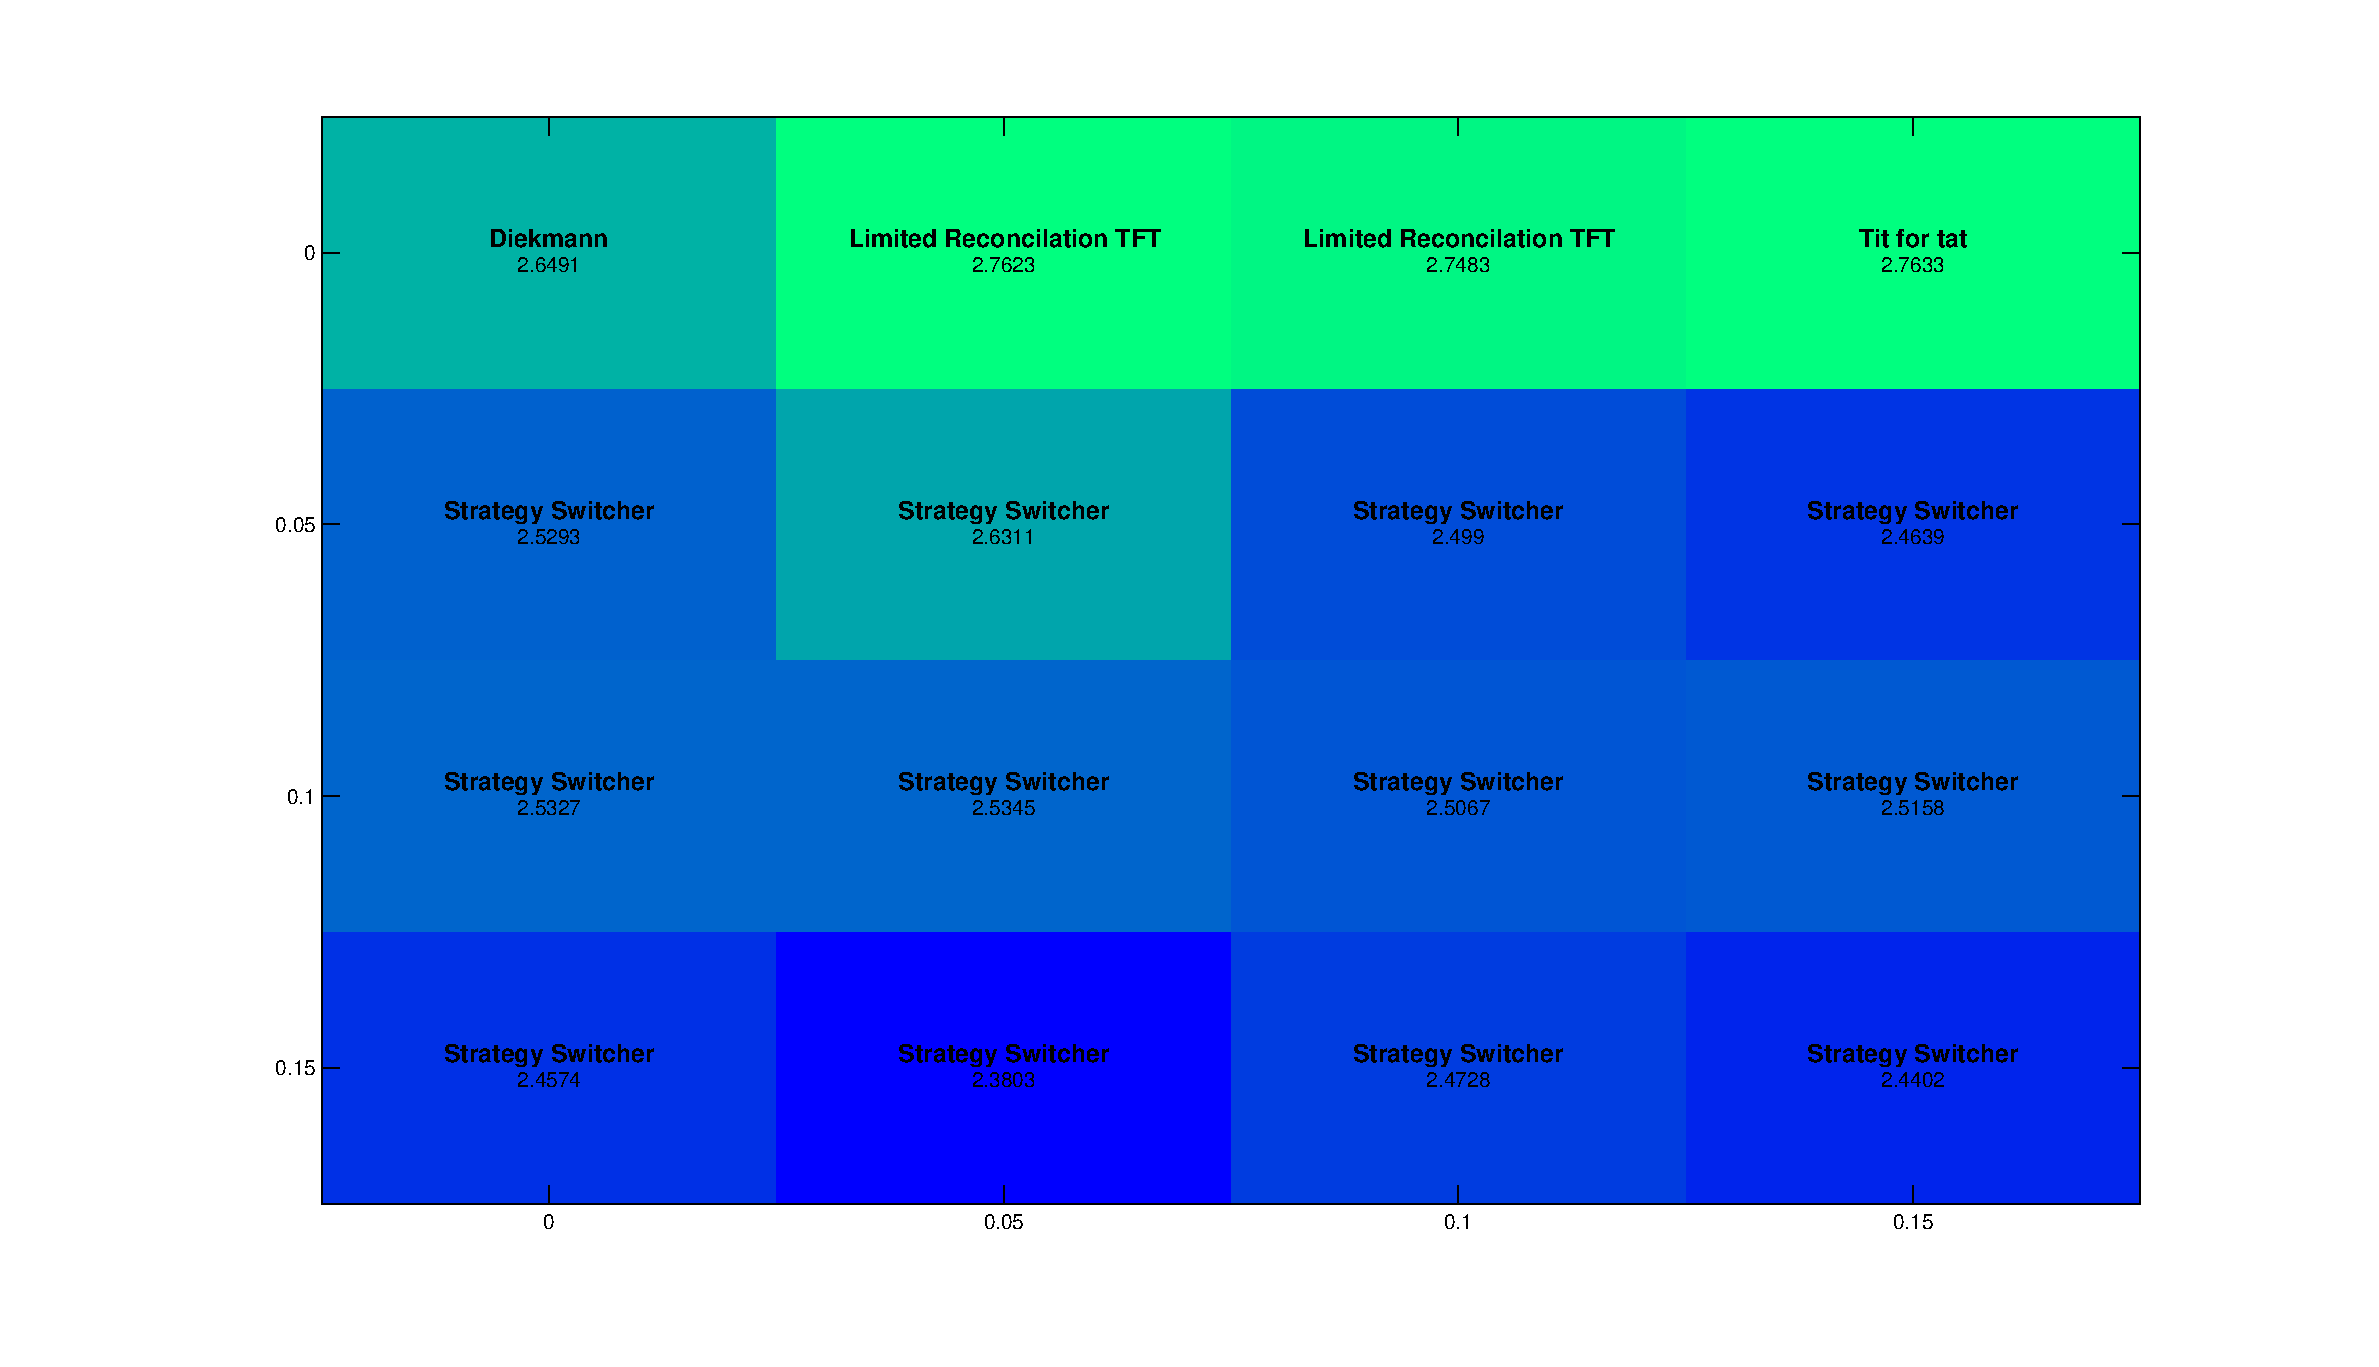
\includegraphics[width=\textwidth]{pics/simulation1/Reward_vs_Noise_with_best_Player_named}}
\end{minipage}

\begin{minipage}[hbt]{1\textwidth}
	\centering
	\subfloat[Simulation 2]{\label{fig:simul2namedplayer}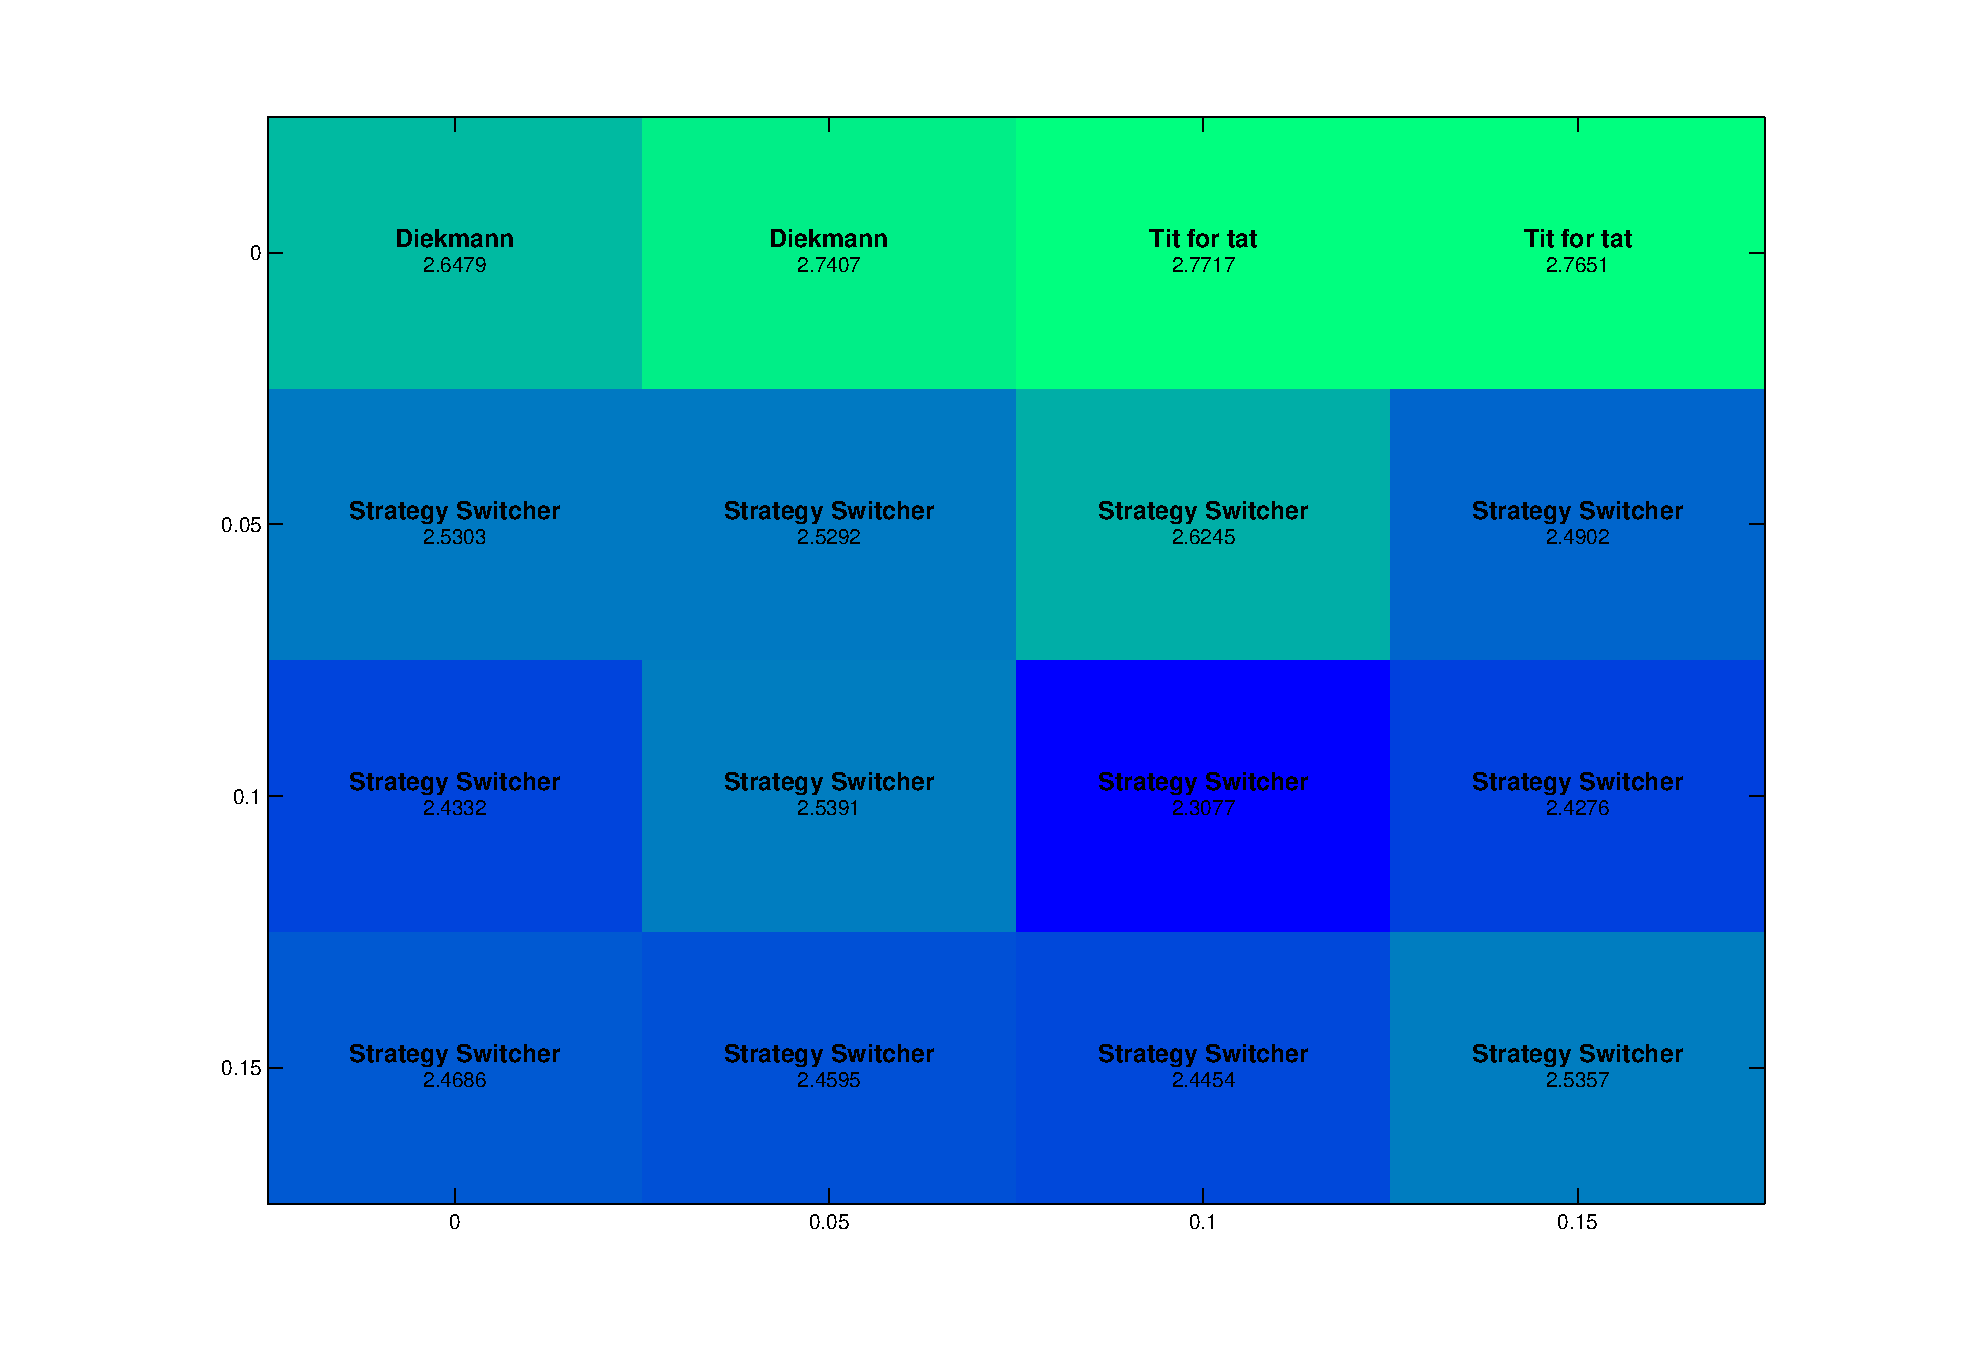
\includegraphics[width=0.9\textwidth]{pics/simulation2/Reward_vs_Noise_with_best_Player_named}}
\end{minipage}	
\end{figure}

At noise1 equal zero the \verb0TFT0 mutants win, but for every noise1 larger than zero \verb0SSW0 wins, due to the small impact the noise has on his performance. For noise levels even bigger always defect will be the best strategy.\clearpage

The graphs~\ref{pic player noise1},~\ref{pic player noise2},~\ref{pic player noise3} and~\ref{pic player noise4} illustrate the player's performances compared at different noise levels.\\


\begin{figure}[h]
	\caption{Comparison of all players at zero noise}
	\label{pic player noise1}
\begin{minipage}[hbt]{0.68\textwidth}
	\centering
	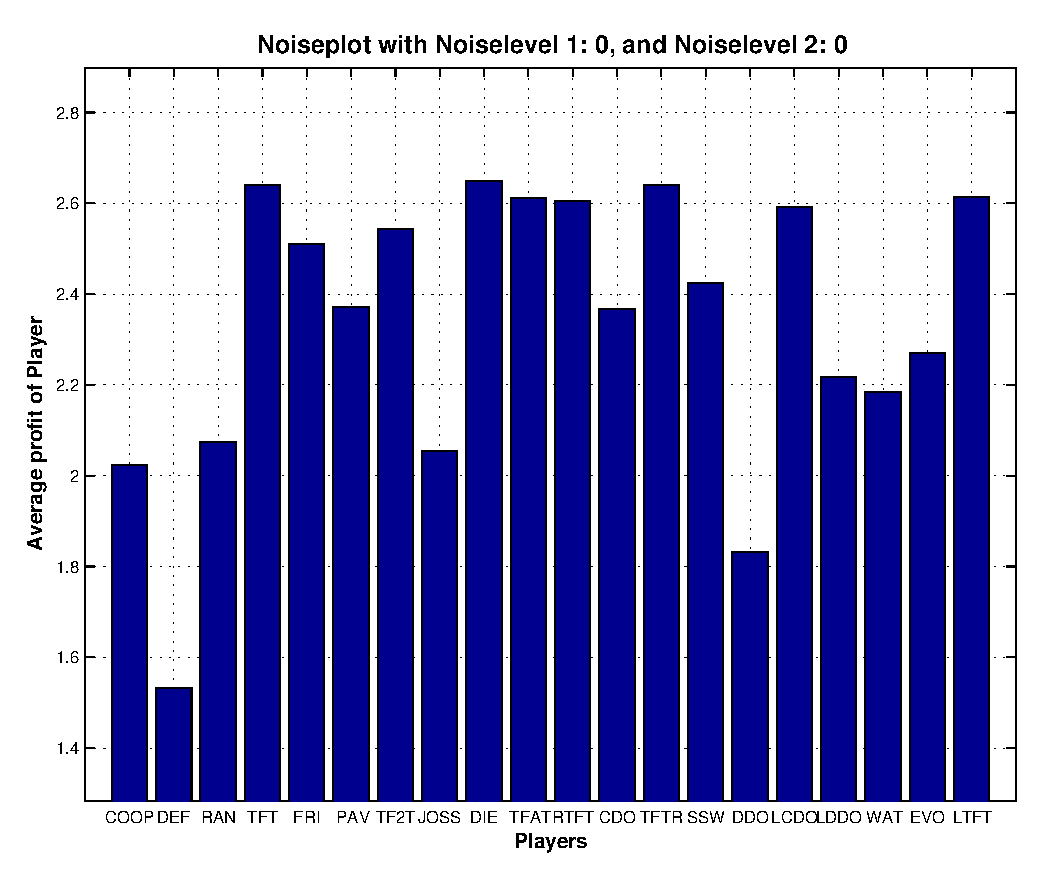
\includegraphics[width=\textwidth]{pics/simulation1/Reward_of__all_Players_at_given_Noiselevels_1}
\end{minipage}
\hfill
\begin{minipage}[hbt]{0.3\textwidth}
	\centering
	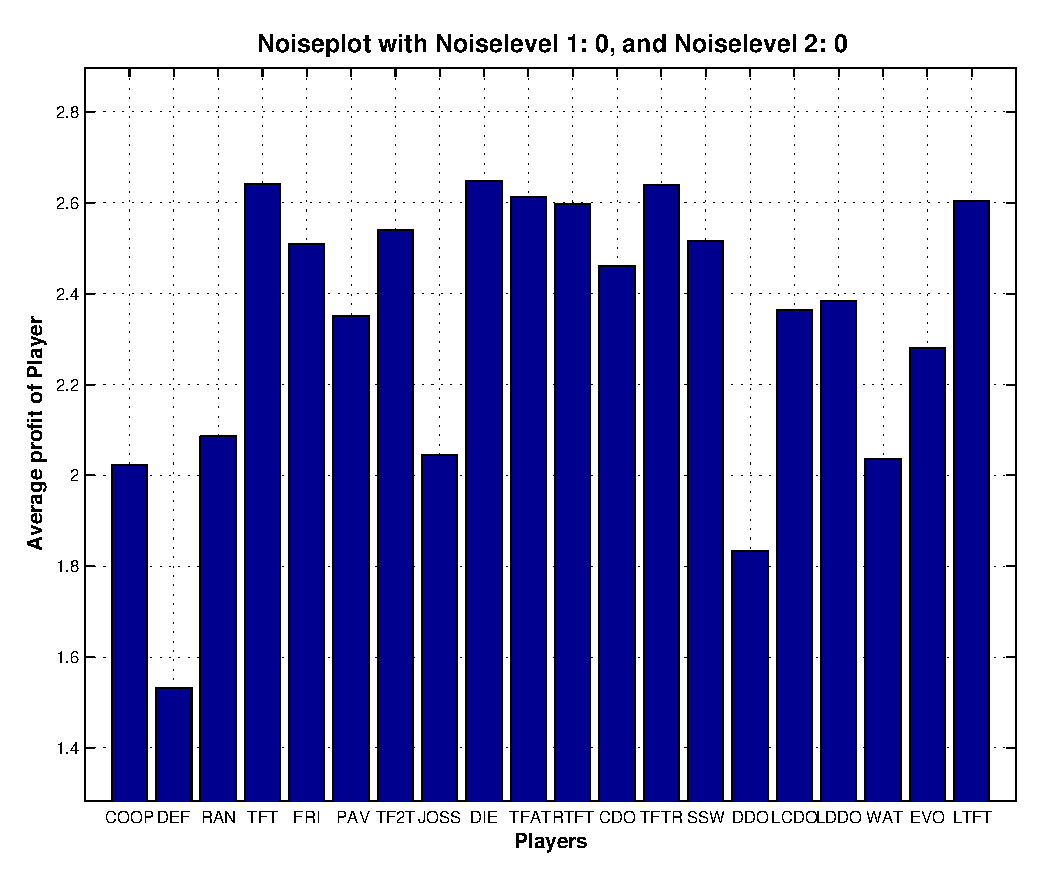
\includegraphics[width=\textwidth]{pics/simulation2/Reward_of_all_Players_at_given_Noiselevels_1}
\end{minipage}
\end{figure}

With no noise the best strategies are either \verb0TFT0 mutants, or variants of \verb0CDO0. Defective strategies perform poorly, which is in accordance to what Axelrod said: “be nice”.\\

\begin{figure}[h]
	\caption{Comparison at noise1 equal to zero and noise2 = 0.1}
	\label{pic player noise2}
\begin{minipage}[hbt]{0.68\textwidth}
	\centering
	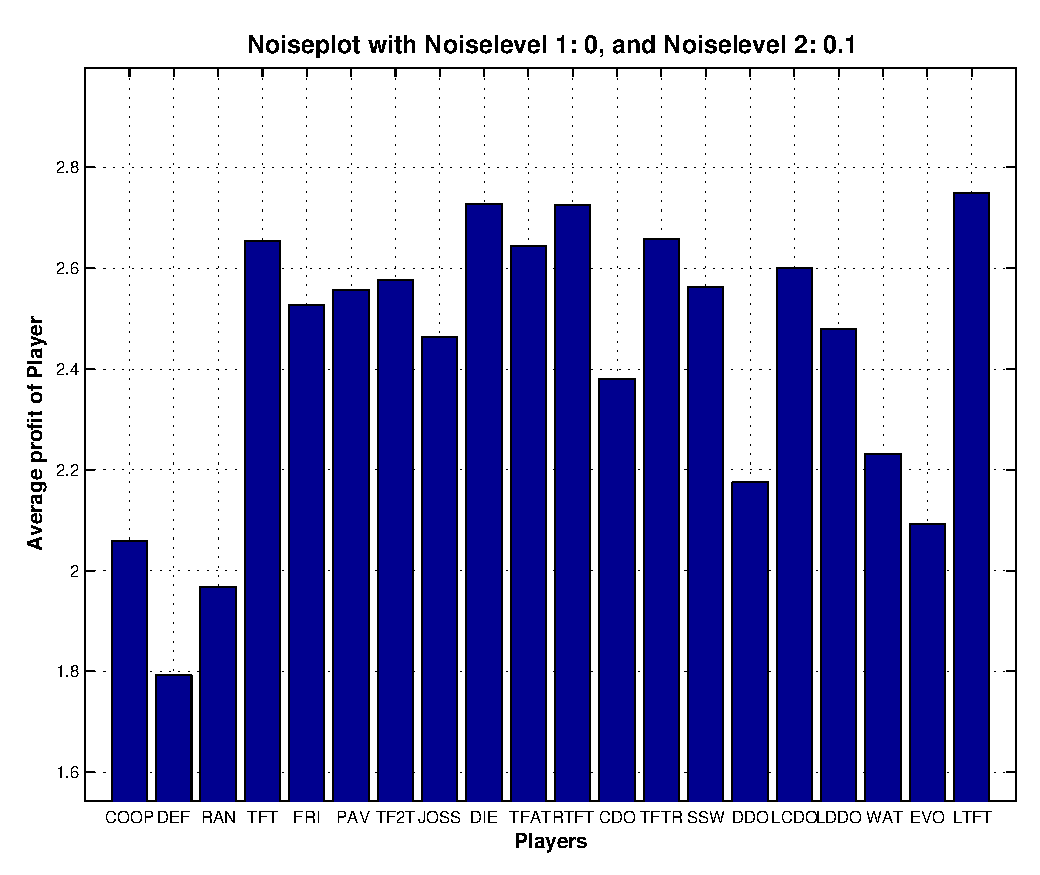
\includegraphics[width=\textwidth]{pics/simulation1/Reward_of_all_Players_at_given_Noiselevels_2}
\end{minipage}
\hfill
\begin{minipage}[hbt]{0.3\textwidth}
	\centering
	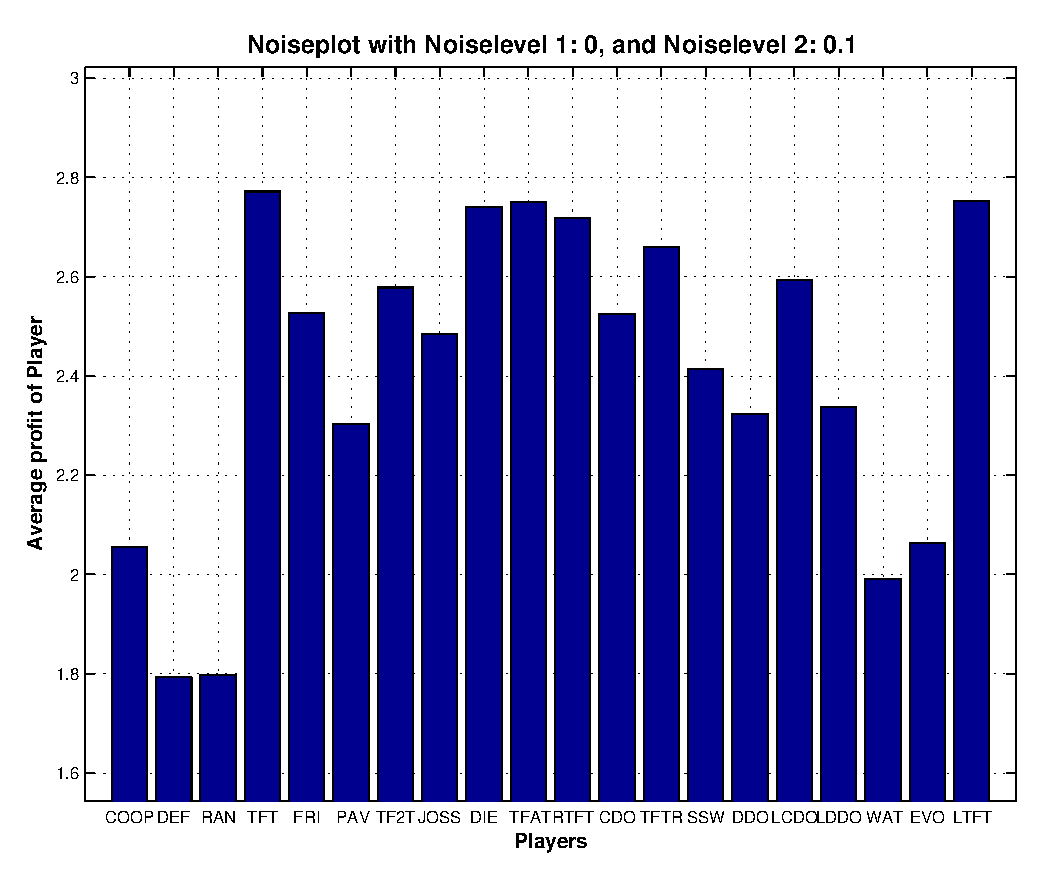
\includegraphics[width=\textwidth]{pics/simulation2/Reward_of_all_Players_at_given_Noiselevels_2}
\end{minipage}
\end{figure}

Figure~\ref{pic player noise2} indicate, that the ranking of the different strategies does not change much. Generally everybody is profiting of the noise, because some defections are now transmitted as cooperations and the whole setup gets more reward.\\

\begin{figure}[h]
\caption{Comparison at noise2 equal to zero and noise1 = 0.1}
	\label{pic player noise3}
\begin{minipage}[hbt]{0.68\textwidth}
	\centering
	\includegraphics[width=\textwidth]{pics/simulation1/Reward_of_all_Players_at_given_Noiselevels_3}
\end{minipage}
\hfill
\begin{minipage}[hbt]{0.3\textwidth}
	\centering
	\includegraphics[width=\textwidth]{pics/simulation2/Reward_of_all_Players_at_given_Noiselevels_3}
\end{minipage}	
\end{figure}

In figure~\ref{pic player noise3} it is obvious, that the performance of the \verb0TFT0 mutants drastically decreases. Only \verb0DIE0 stays somewhat high. The strongest strategies are now the looking back Downings and \verb0SS0. Before, \verb0SS0 had the problem, that the defections he tried out, to exploit non-responding players cost him a lot. Now everybody sees more defections due to the noise, that actually are really taken, and it doesn’t matter that much anymore.\\

\begin{figure}[h]
\caption{Comparison at noise2 and noise1 = 0.1}
	\label{pic player noise4}
\begin{minipage}[hbt]{0.68\textwidth}
	\centering
	\includegraphics[width=\textwidth]{pics/simulation1/Reward_of_all_Players_at_given_Noiselevels_4}
\end{minipage}
\hfill
\begin{minipage}[hbt]{0.3\textwidth}
	\centering
	\includegraphics[width=\textwidth]{pics/simulation2/Reward_of_all_Players_at_given_Noiselevels_4}
\end{minipage}	
\end{figure}

In figure~\ref{pic player noise4} the \verb0TFT0 mutants perform somewhat better than without noise2, but \verb0SS0 is still much stronger than all the other players.




